\chapter{\texorpdfstring{$\delta_{metric}$}{delta} Plots}
\label{ape:delta-plots}

Texto texto texto texto texto texto texto texto texto texto texto texto texto
texto texto texto texto texto texto texto texto texto texto texto texto texto
texto texto texto texto texto texto.


\singlespacing

\renewcommand{\arraystretch}{0.85}
\captionsetup{margin=1.0cm}  % correção nas margens dos captions.
%--------------------------------------------------------------------------------------

\begin{figure}[H]
    \centering
    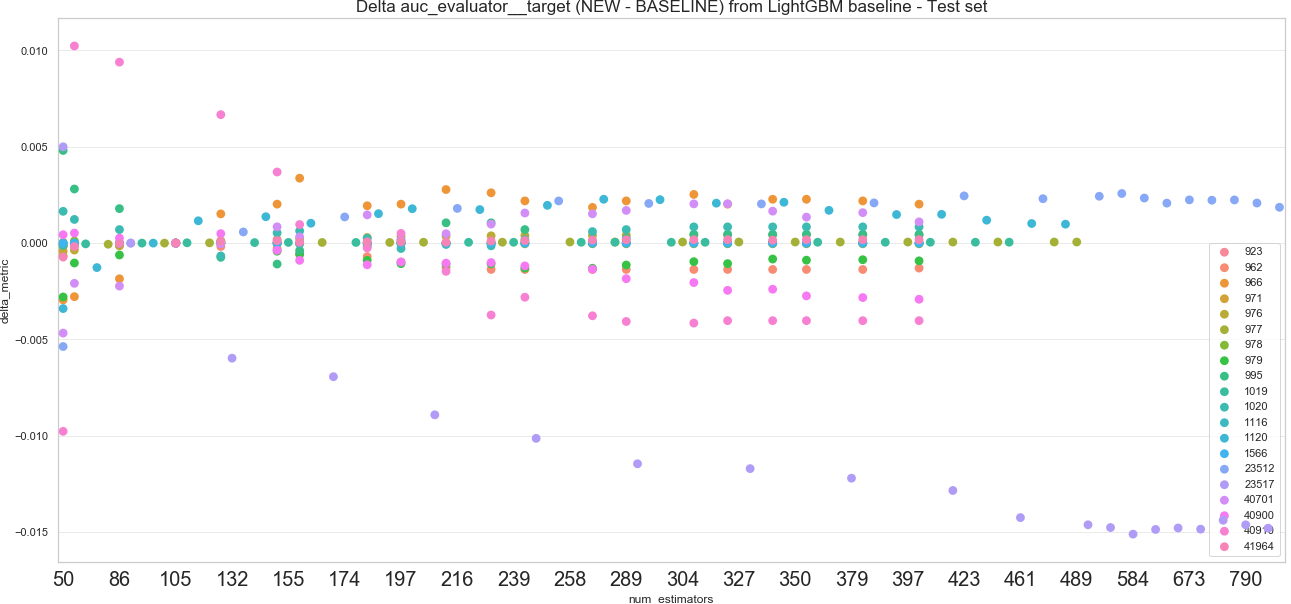
\includegraphics[width=.75\textwidth]{appendix_figures/delta_auc_cluster1_num_estimators.png}
    \caption{$\delta_{AUC}$ plot for $\mathcal{S}(C_1, \eta^{(1)}_{NE}, AUC)$}
\end{figure}


% \begin{figure}[H]
%     \centering
%     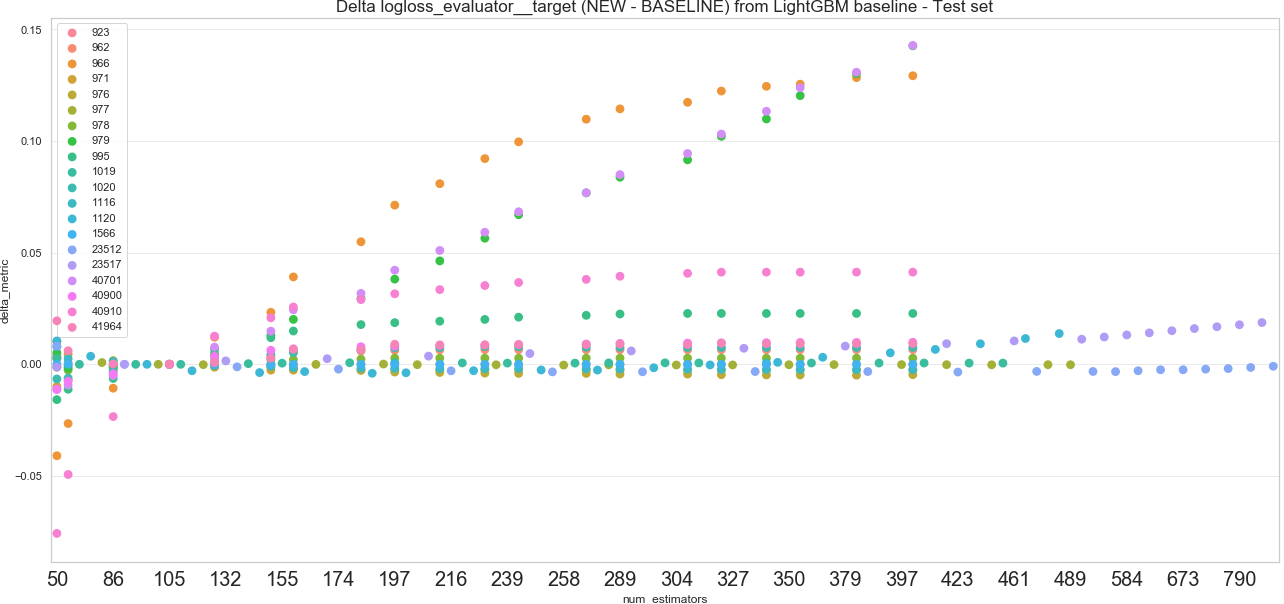
\includegraphics[width=.75\textwidth]{appendix_figures/delta_logloss_cluster1_num_estimators.png}
%     \caption{$\delta_{Logloss}$ plot for $\mathcal{S}(C_1, \eta^{(1)}_{NE}, Logloss)$}
% \end{figure}


% \begin{figure}[H]
%     \centering
%     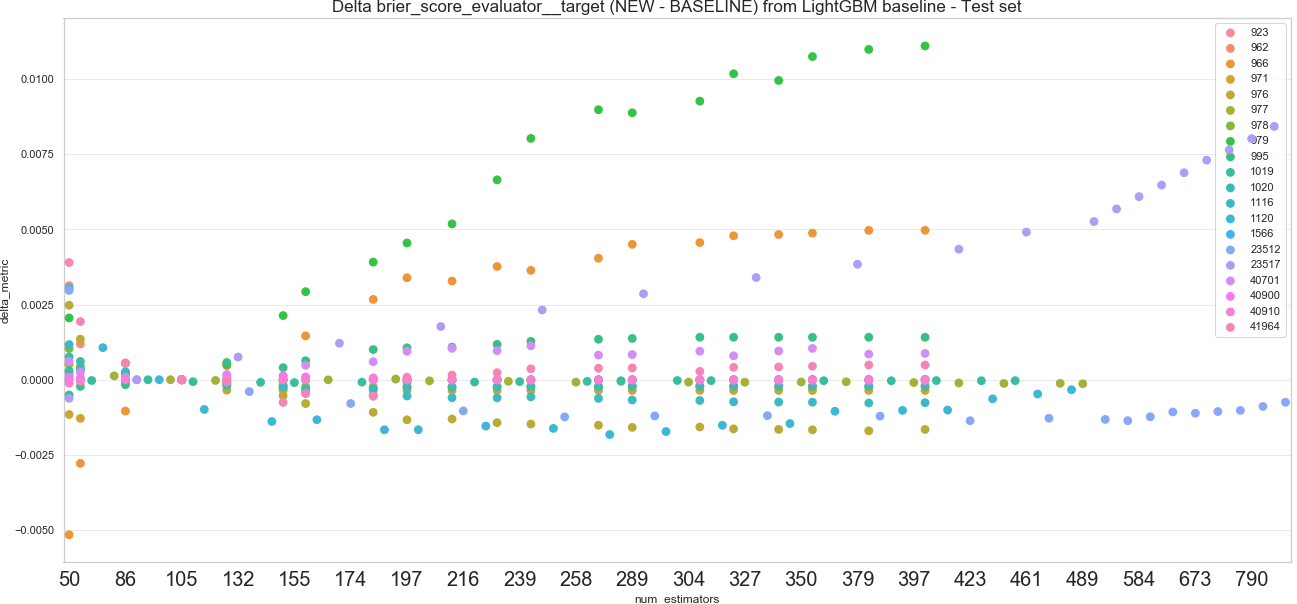
\includegraphics[width=.75\textwidth]{appendix_figures/delta_brier_cluster1_num_estimators.png}
%     \caption{$\delta_{Brier}$ plot for $\mathcal{S}(C_1, \eta^{(1)}_{NE}, Brier)$}
% \end{figure}


% \begin{figure}[H]
%     \centering
%     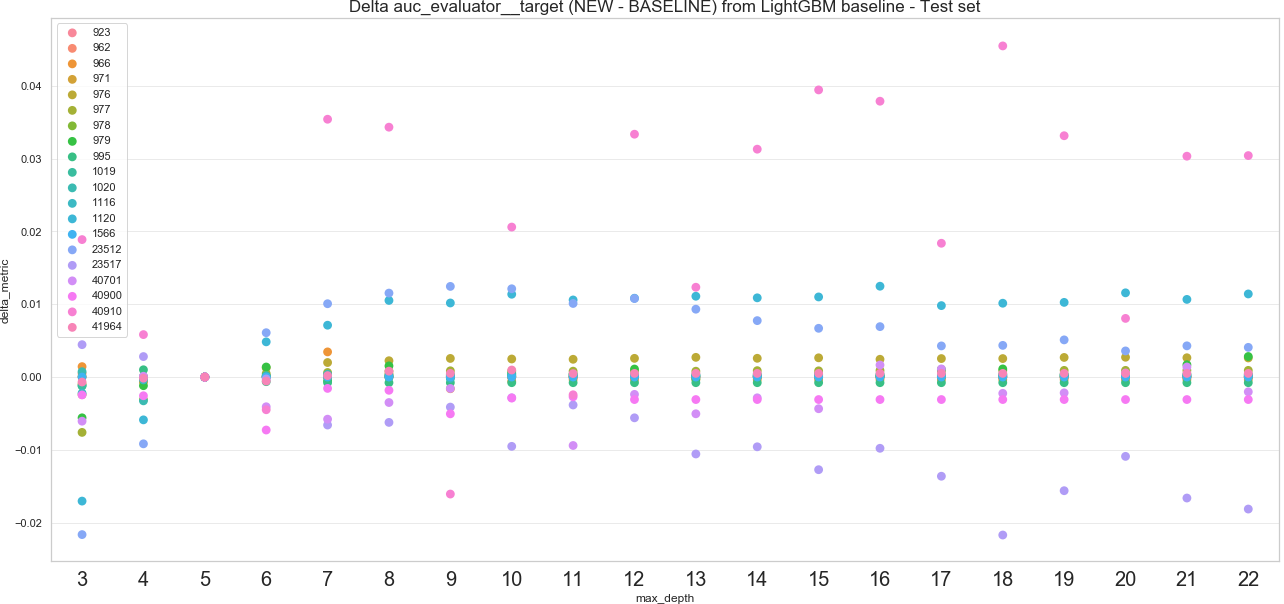
\includegraphics[width=.75\textwidth]{appendix_figures/delta_auc_cluster1_max_depth.png}
%     \caption{$\delta_{AUC}$ plot for $\mathcal{S}(C_1, \eta^{(1)}_{MD}, AUC)$}
% \end{figure}


% \begin{figure}[H]
%     \centering
%     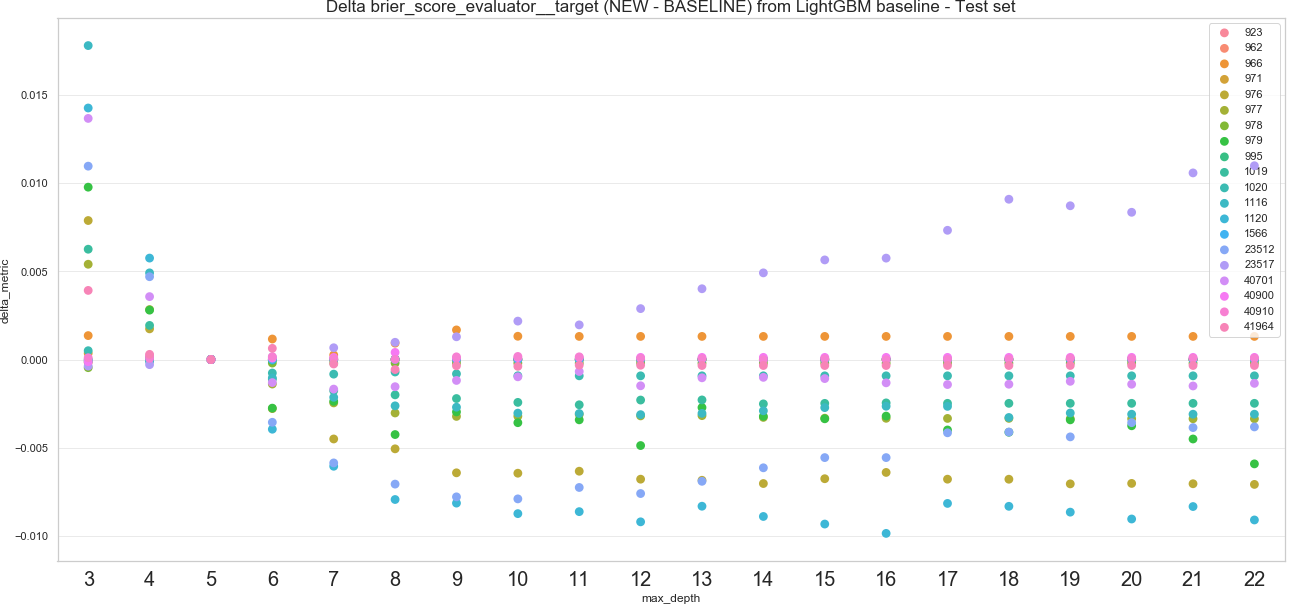
\includegraphics[width=.75\textwidth]{appendix_figures/delta_brier_cluster1_max_depth.png}
%     \caption{$\delta_{Brier}$ plot for $\mathcal{S}(C_1, \eta^{(1)}_{MD}, Brier)$}
% \end{figure}


% \begin{figure}[H]
%     \centering
%     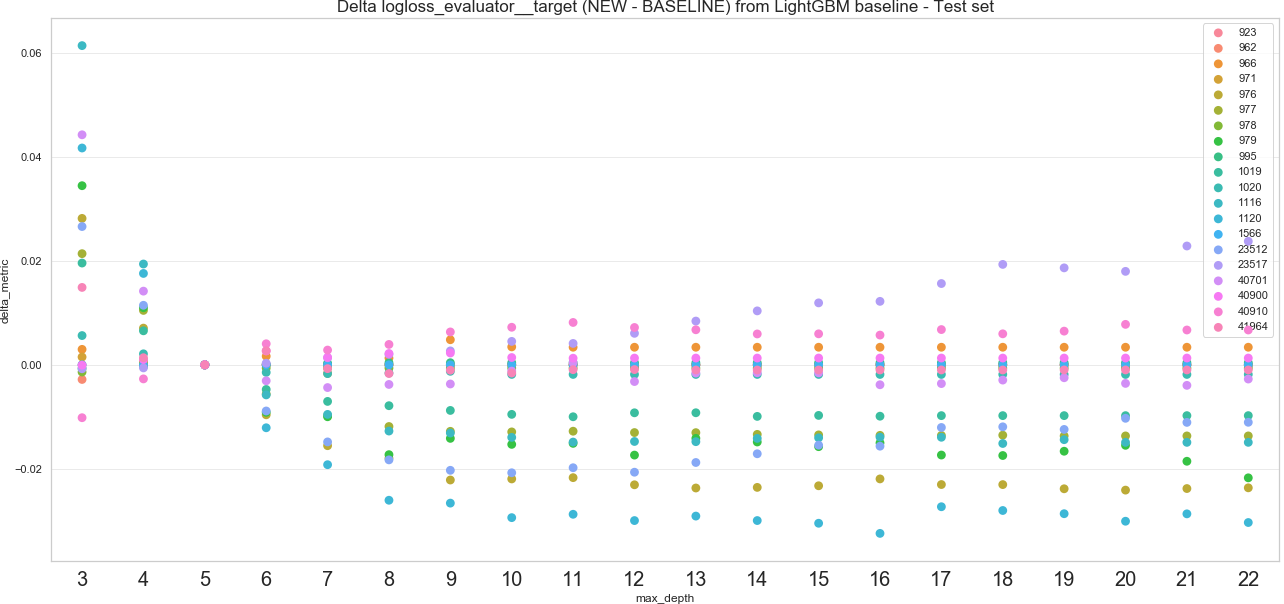
\includegraphics[width=.75\textwidth]{appendix_figures/delta_logloss_cluster1_max_depth.png}
%     \caption{$\delta_{Logloss}$ plot for $\mathcal{S}(C_1, \eta^{(1)}_{MD}, Logloss)$}
% \end{figure}


% \begin{figure}[H]
%     \centering
%     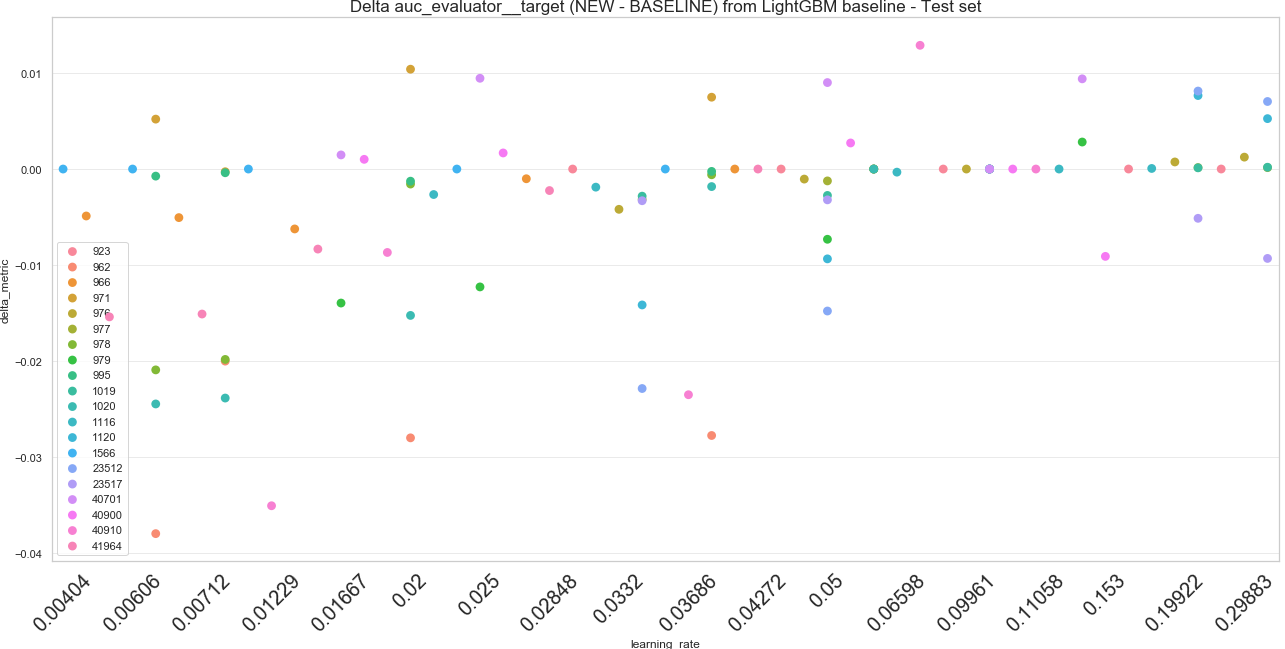
\includegraphics[width=.75\textwidth]{appendix_figures/delta_auc_cluster1_learning_rate.png}
%     \caption{$\delta_{AUC}$ plot for $\mathcal{S}(C_1, \eta^{(1)}_{LR}, AUC)$}
% \end{figure}


% \begin{figure}[H]
%     \centering
%     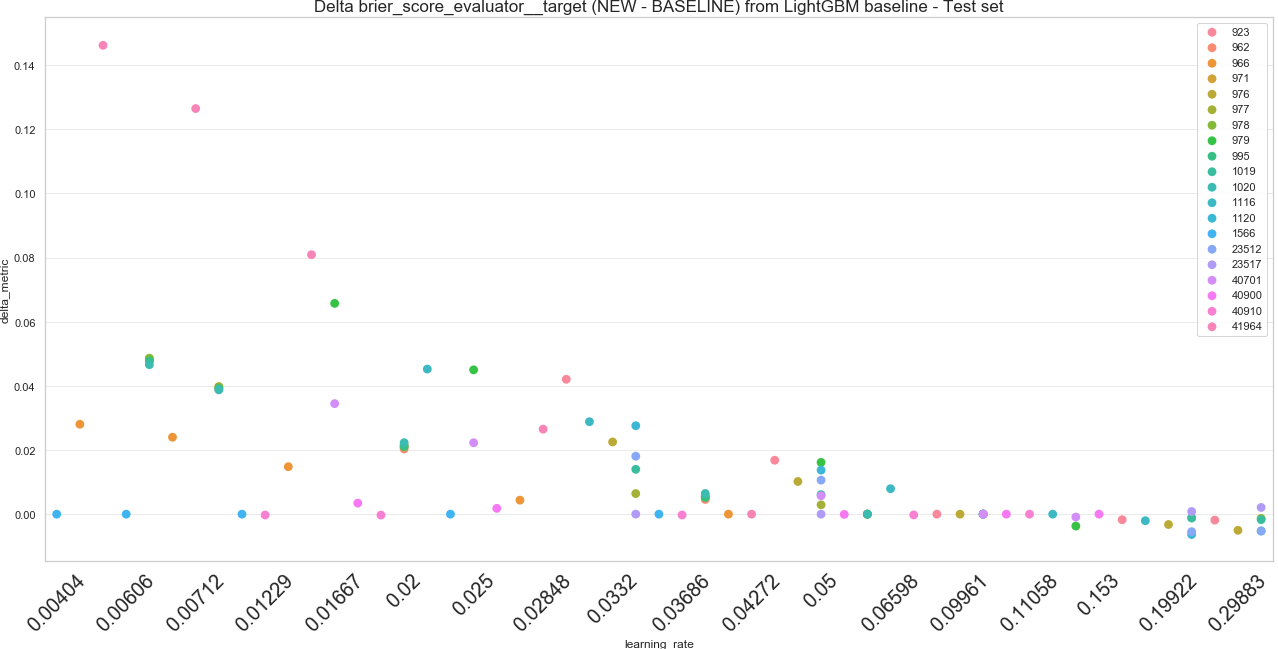
\includegraphics[width=.75\textwidth]{appendix_figures/delta_brier_cluster1_learning_rate.png}
%     \caption{$\delta_{Brier}$ plot for $\mathcal{S}(C_1, \eta^{(1)}_{LR}, Brier)$}
% \end{figure}


% \begin{figure}[H]
%     \centering
%     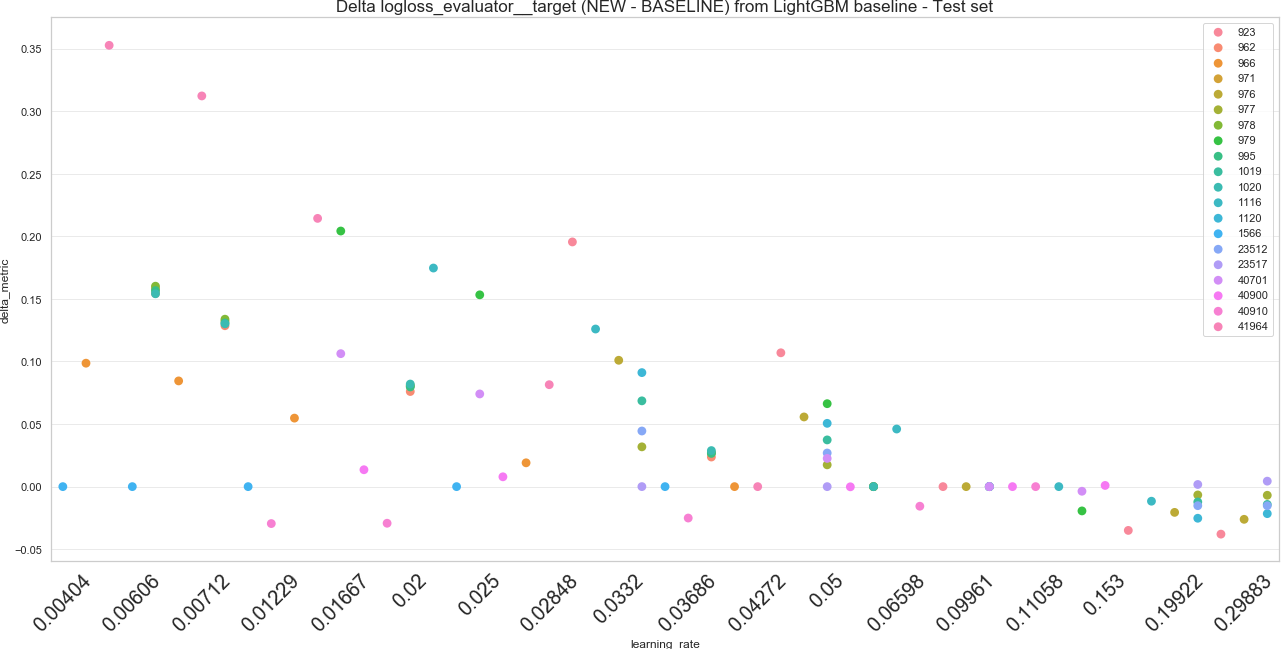
\includegraphics[width=.75\textwidth]{appendix_figures/delta_logloss_cluster1_learning_rate.png}
%     \caption{$\delta_{Logloss}$ plot for $\mathcal{S}(C_1, \eta^{(1)}_{LR}, Logloss)$}
% \end{figure}


% \begin{figure}[H]
%     \centering
%     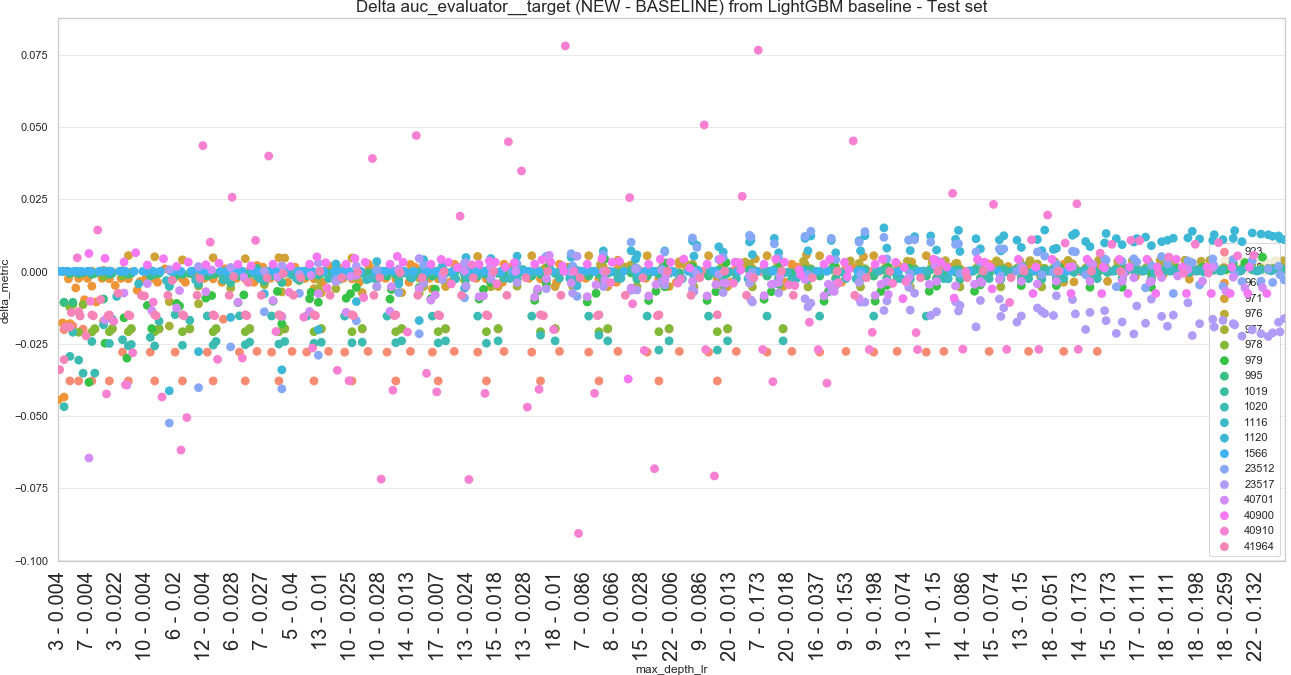
\includegraphics[width=.75\textwidth]{appendix_figures/delta_auc_cluster1_max_depth_lr.png}
%     \caption{$\delta_{AUC}$ plot for $\mathcal{S}(C_1, \eta^{(1)}_{MD, LR}, AUC)$}
% \end{figure}


% \begin{figure}[H]
%     \centering
%     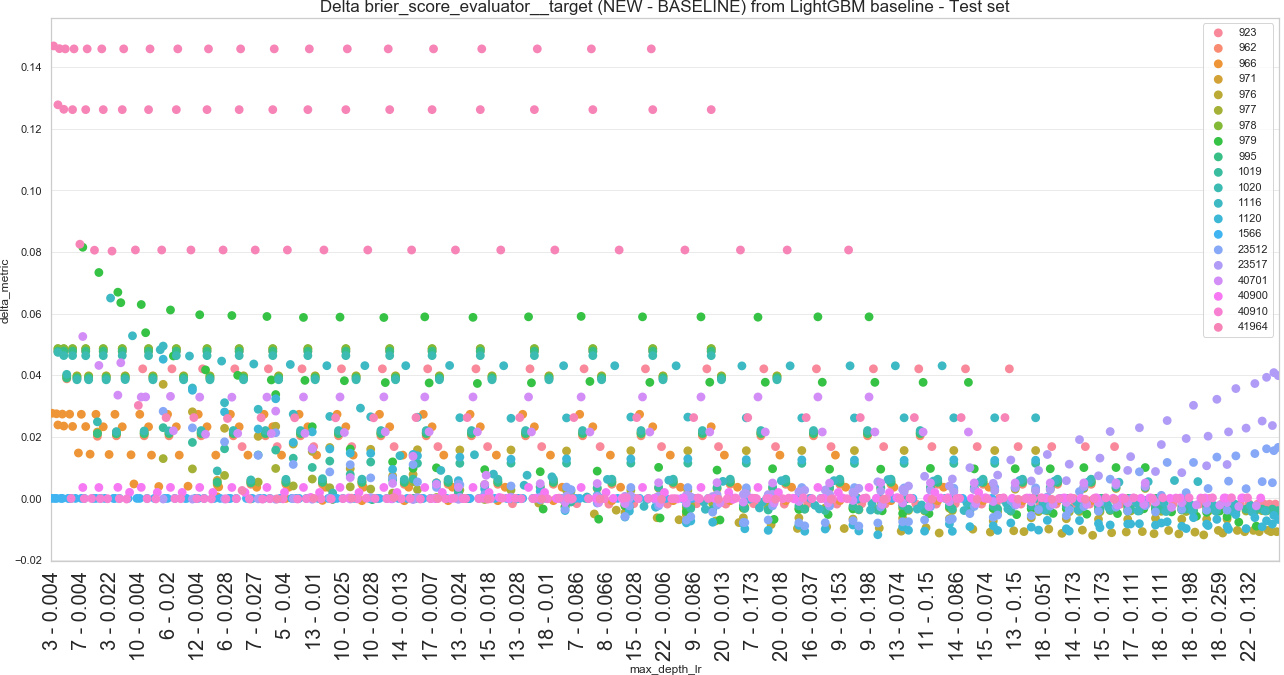
\includegraphics[width=.75\textwidth]{appendix_figures/delta_brier_cluster1_max_depth_lr.png}
%     \caption{$\delta_{Brier}$ plot for $\mathcal{S}(C_1, \eta^{(1)}_{MD, LR}, Brier)$}
% \end{figure}


% \begin{figure}[H]
%     \centering
%     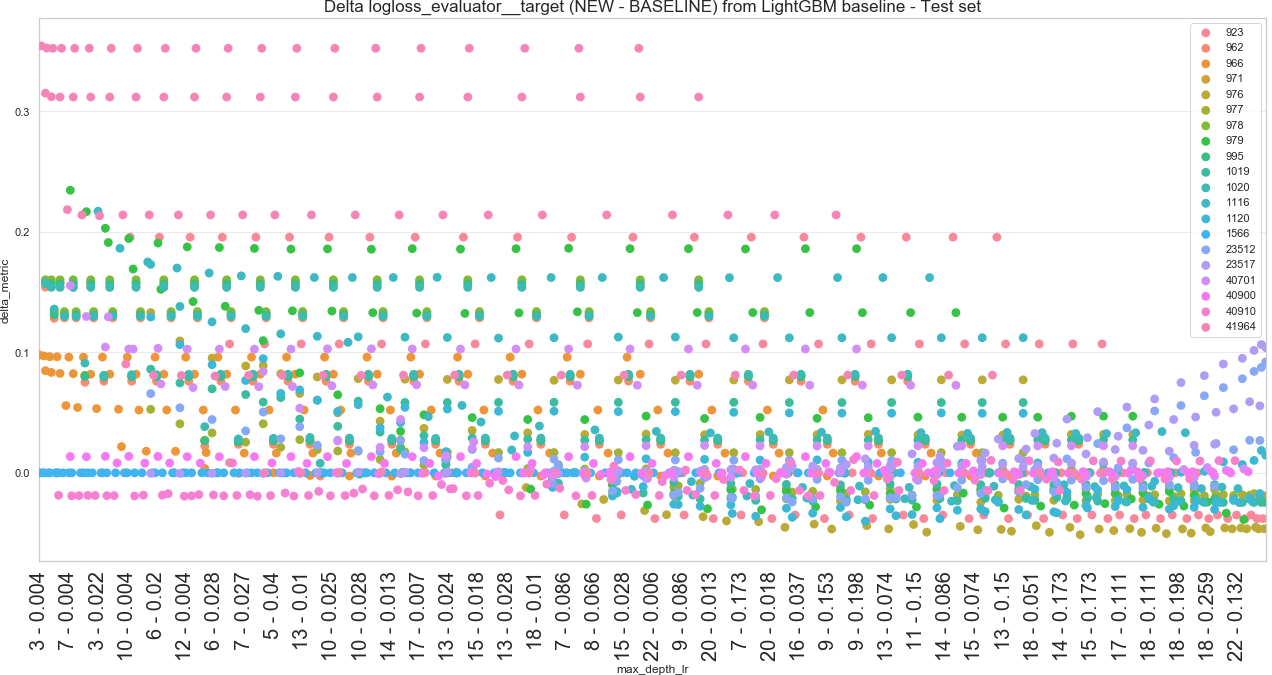
\includegraphics[width=.75\textwidth]{appendix_figures/delta_logloss_cluster1_max_depth_lr.png}
%     \caption{$\delta_{Logloss}$ plot for $\mathcal{S}(C_1, \eta^{(1)}_{MD, LR}, Logloss)$}
% \end{figure}


% \begin{figure}[H]
%     \centering
%     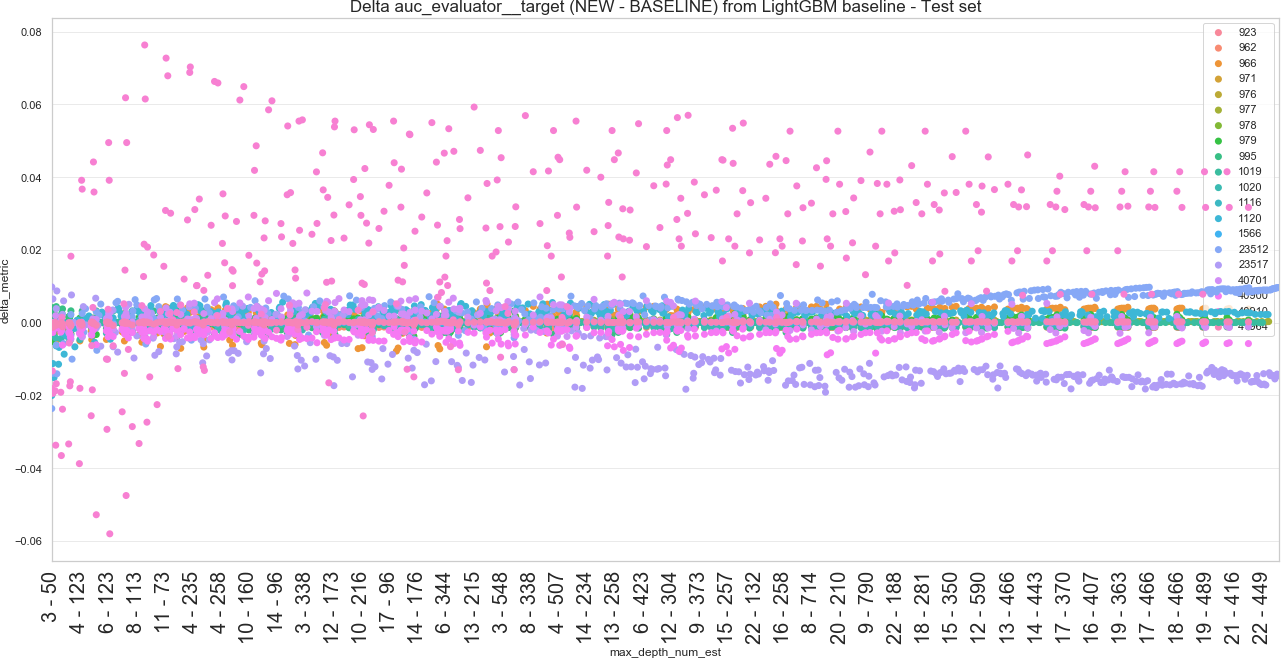
\includegraphics[width=.75\textwidth]{appendix_figures/delta_auc_cluster1_max_depth_num_est.png}
%     \caption{$\delta_{AUC}$ plot for $\mathcal{S}(C_1, \eta^{(1)}_{MD, NE}, AUC)$}
% \end{figure}


% \begin{figure}[H]
%     \centering
%     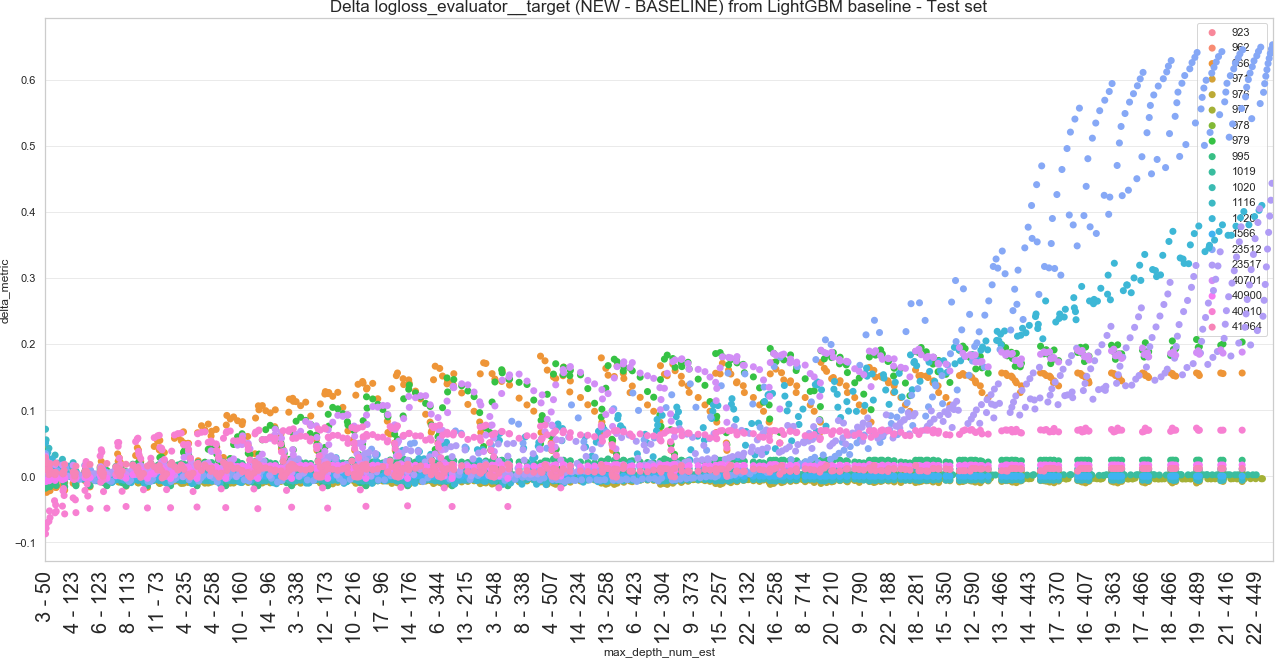
\includegraphics[width=.75\textwidth]{appendix_figures/delta_logloss_cluster1_max_depth_num_est.png}
%     \caption{$\delta_{Logloss}$ plot for $\mathcal{S}(C_1, \eta^{(1)}_{MD, NE}, Logloss)$}
% \end{figure}


% \begin{figure}[H]
%     \centering
%     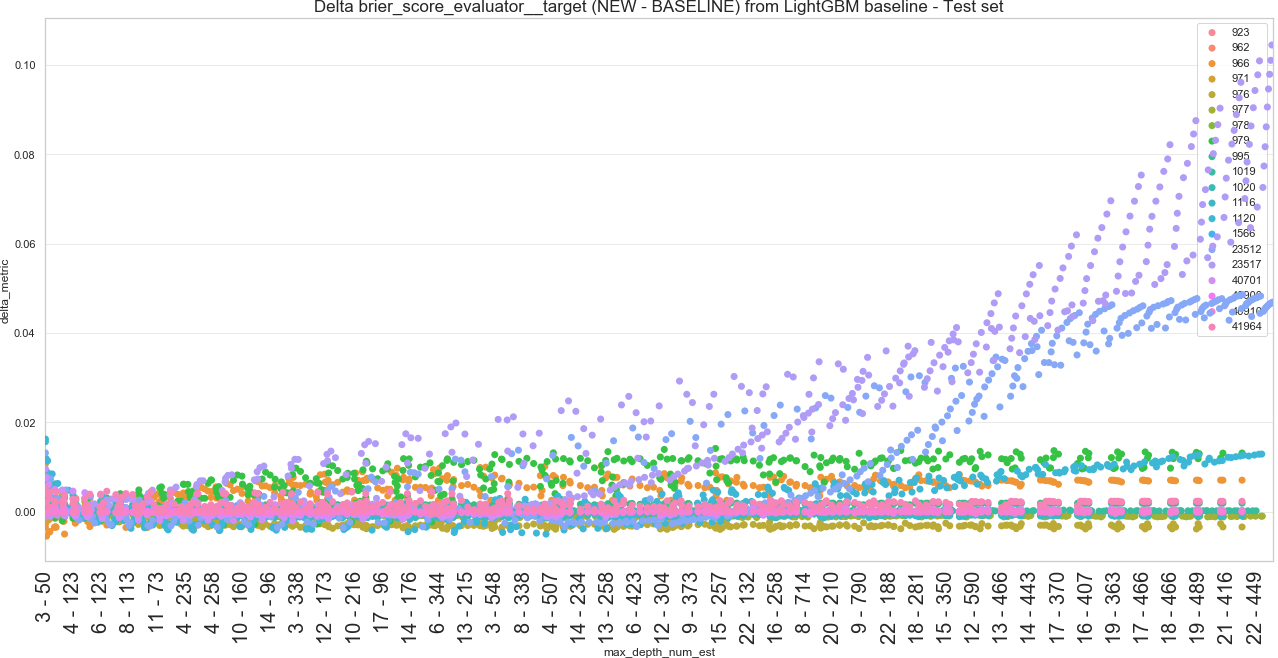
\includegraphics[width=.75\textwidth]{appendix_figures/delta_brier_cluster1_max_depth_num_est.png}
%     \caption{$\delta_{Brier}$ plot for $\mathcal{S}(C_1, \eta^{(1)}_{MD, NE}, Brier)$}
% \end{figure}


% \begin{figure}[H]
%     \centering
%     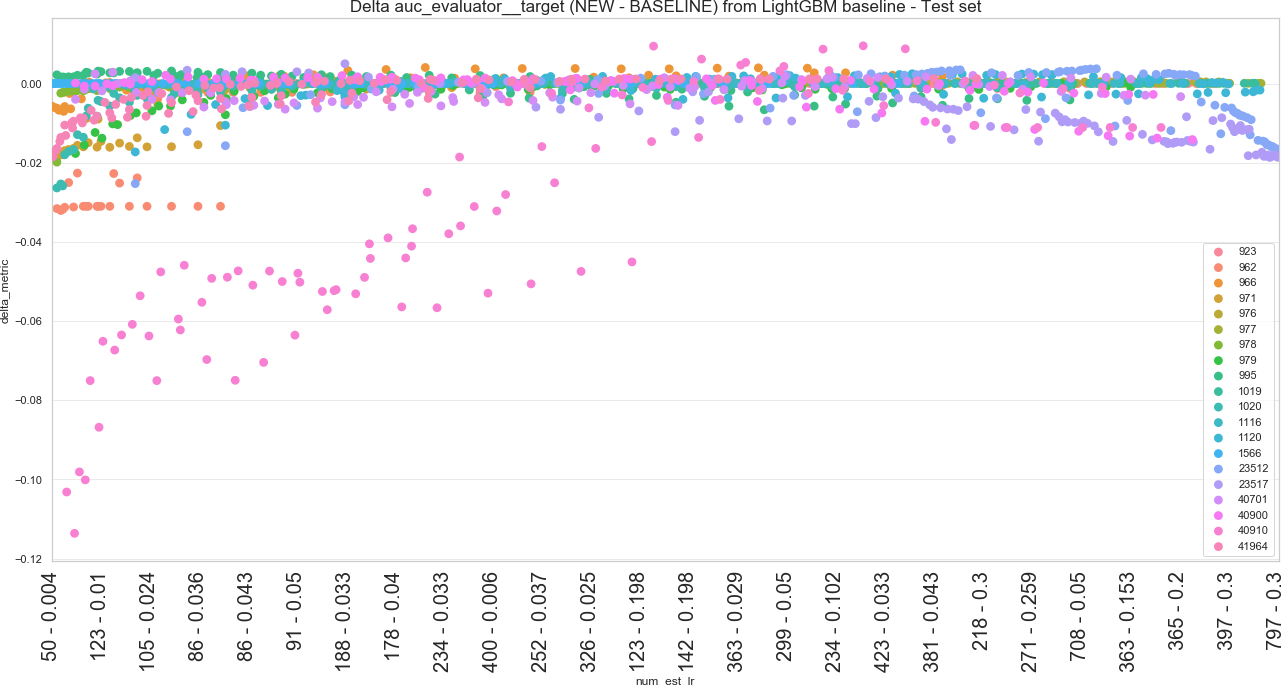
\includegraphics[width=.75\textwidth]{appendix_figures/delta_auc_cluster1_num_est_lr.png}
%     \caption{$\delta_{AUC}$ plot for $\mathcal{S}(C_1, \eta^{(1)}_{LR, NE}, AUC)$}
% \end{figure}


% \begin{figure}[H]
%     \centering
%     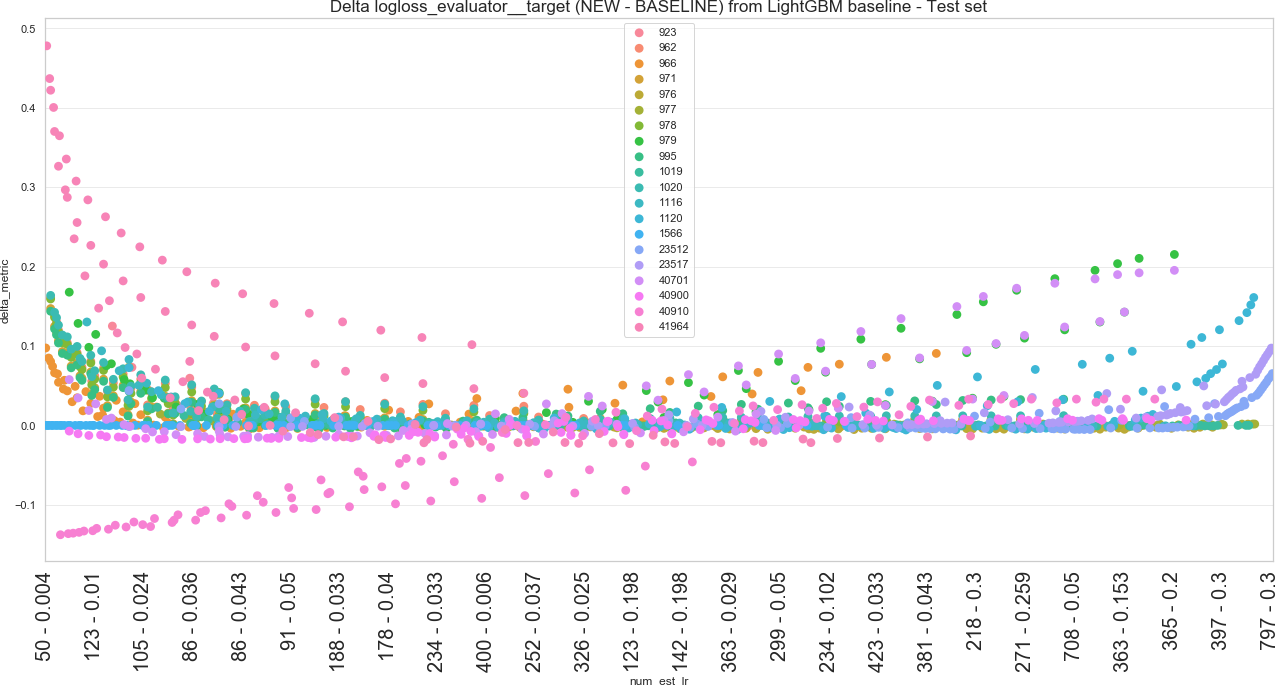
\includegraphics[width=.75\textwidth]{appendix_figures/delta_logloss_cluster1_num_est_lr.png}
%     \caption{$\delta_{Logloss}$ plot for $\mathcal{S}(C_1, \eta^{(1)}_{LR, NE}, Logloss)$}
% \end{figure}


% \begin{figure}[H]
%     \centering
%     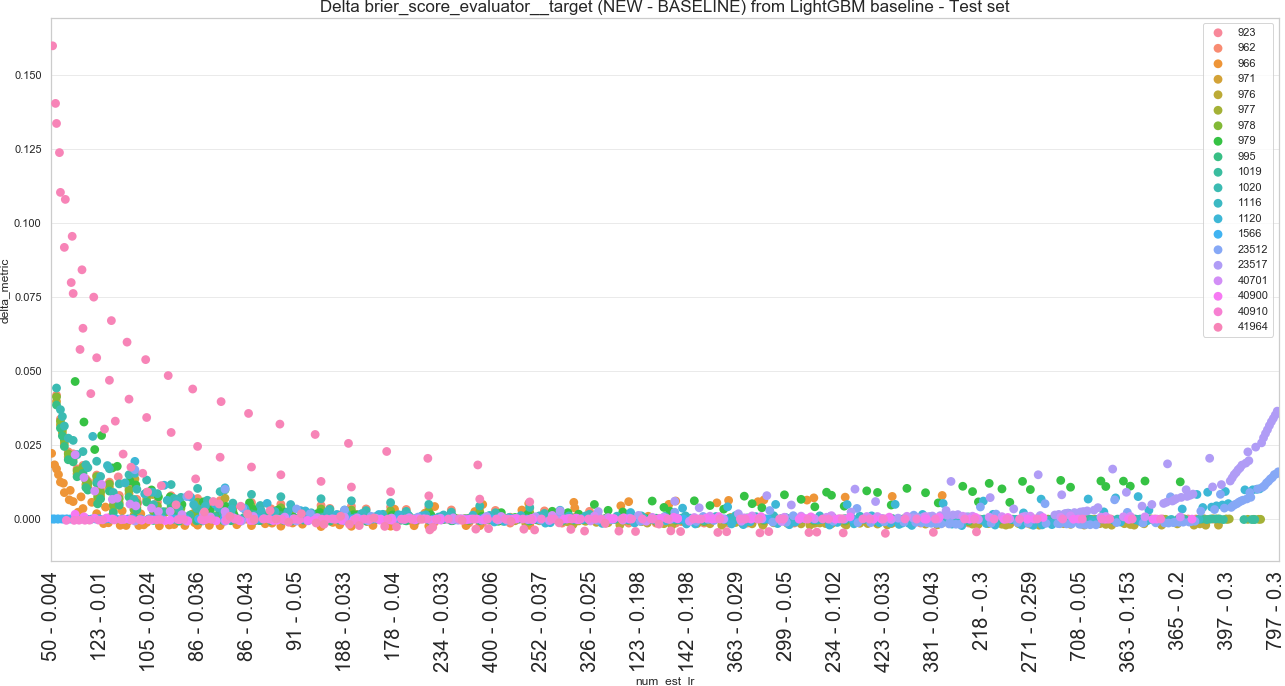
\includegraphics[width=.75\textwidth]{appendix_figures/delta_brier_cluster1_num_est_lr.png}
%     \caption{$\delta_{Brier}$ plot for $\mathcal{S}(C_1, \eta^{(1)}_{LR, NE}, Brier)$}
% \end{figure}


% \begin{figure}[H]
%     \centering
%     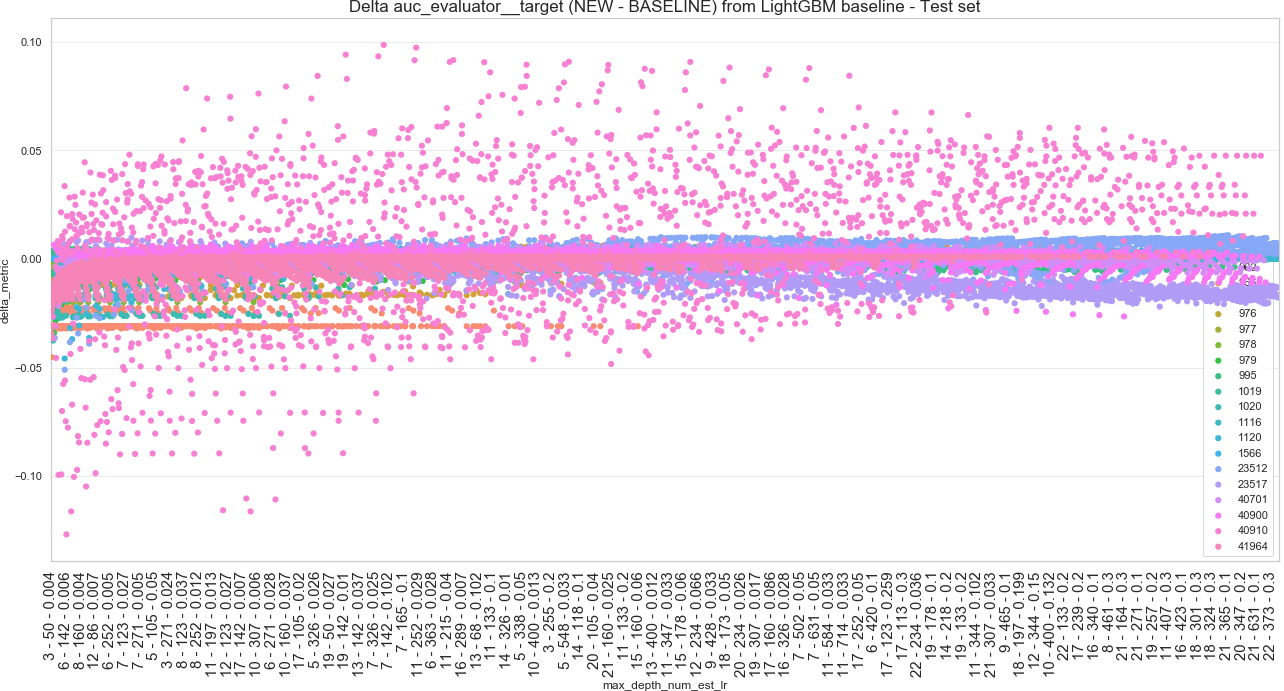
\includegraphics[width=.75\textwidth]{appendix_figures/delta_auc_cluster1_max_depth_num_est_lr.png}
%     \caption{$\delta_{AUC}$ plot for $\mathcal{S}(C_1, \eta^{(1)}_{NE, MD, LR}, AUC)$}
% \end{figure}


% \begin{figure}[H]
%     \centering
%     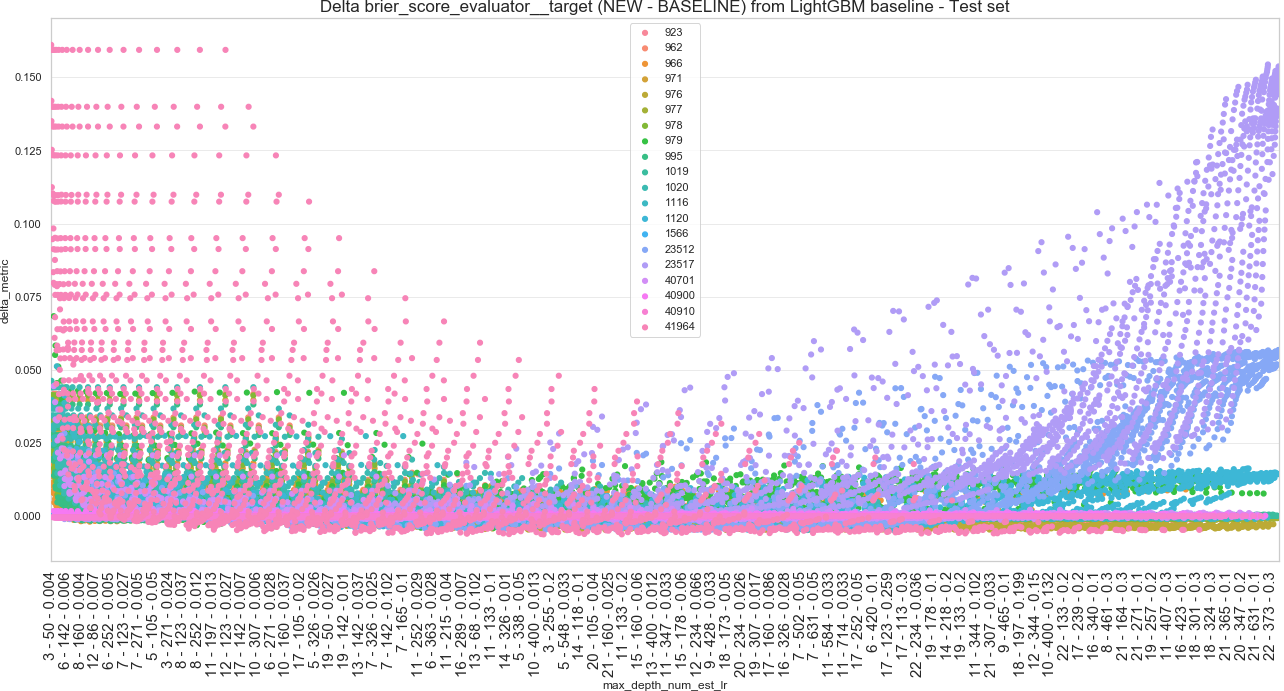
\includegraphics[width=.75\textwidth]{appendix_figures/delta_brier_cluster1_max_depth_num_est_lr.png}
%     \caption{$\delta_{Brier}$ plot for $\mathcal{S}(C_1, \eta^{(1)}_{NE, MD, LR}, Brier)$}
% \end{figure}


% \begin{figure}[H]
%     \centering
%     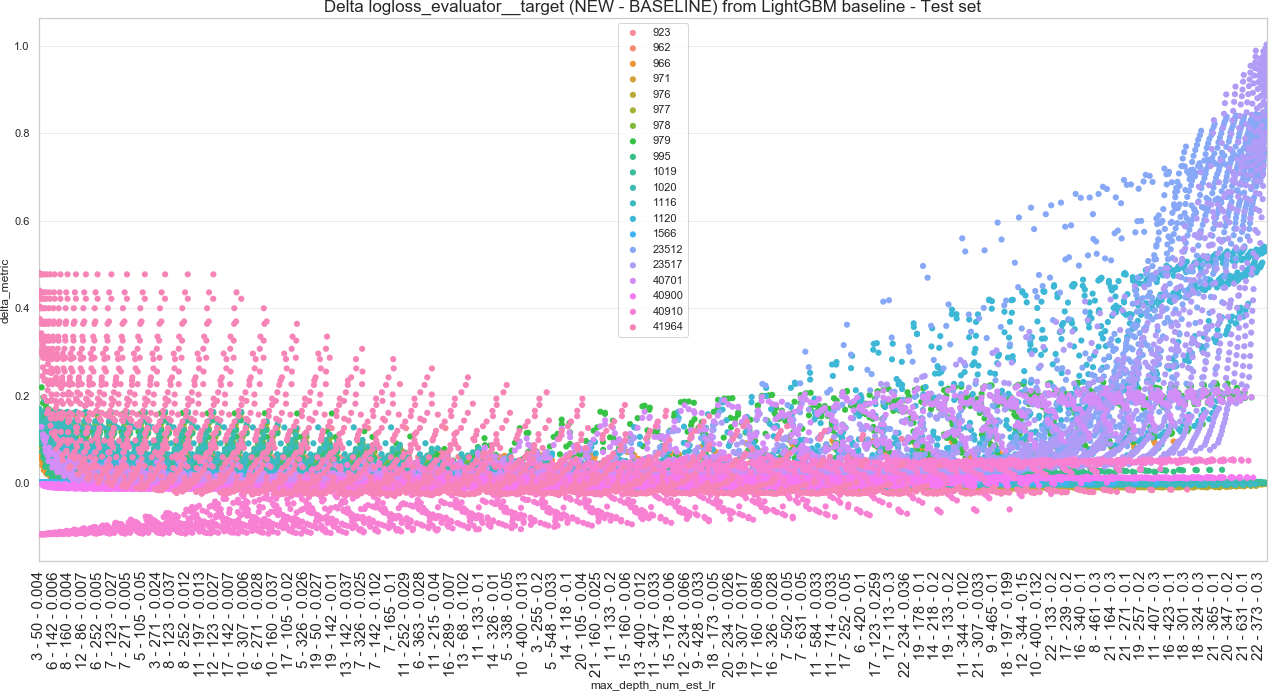
\includegraphics[width=.75\textwidth]{appendix_figures/delta_logloss_cluster1_max_depth_num_est_lr.png}
%     \caption{$\delta_{Logloss}$ plot for $\mathcal{S}(C_1, \eta^{(1)}_{NE, MD, LR}, Logloss)$}
% \end{figure}


% \begin{figure}[H]
%     \centering
%     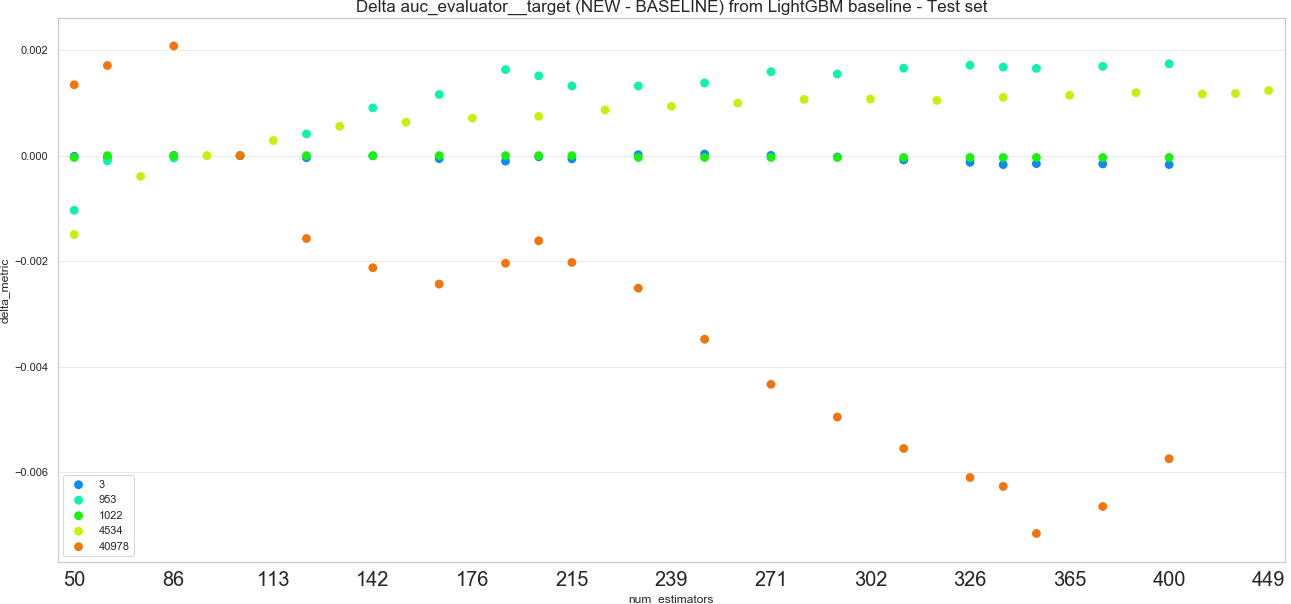
\includegraphics[width=.75\textwidth]{appendix_figures/delta_auc_cluster2_num_estimators.png}
%     \caption{$\delta_{AUC}$ plot for $\mathcal{S}(C_2, \eta^{(2)}_{NE}, AUC)$}
% \end{figure}


% \begin{figure}[H]
%     \centering
%     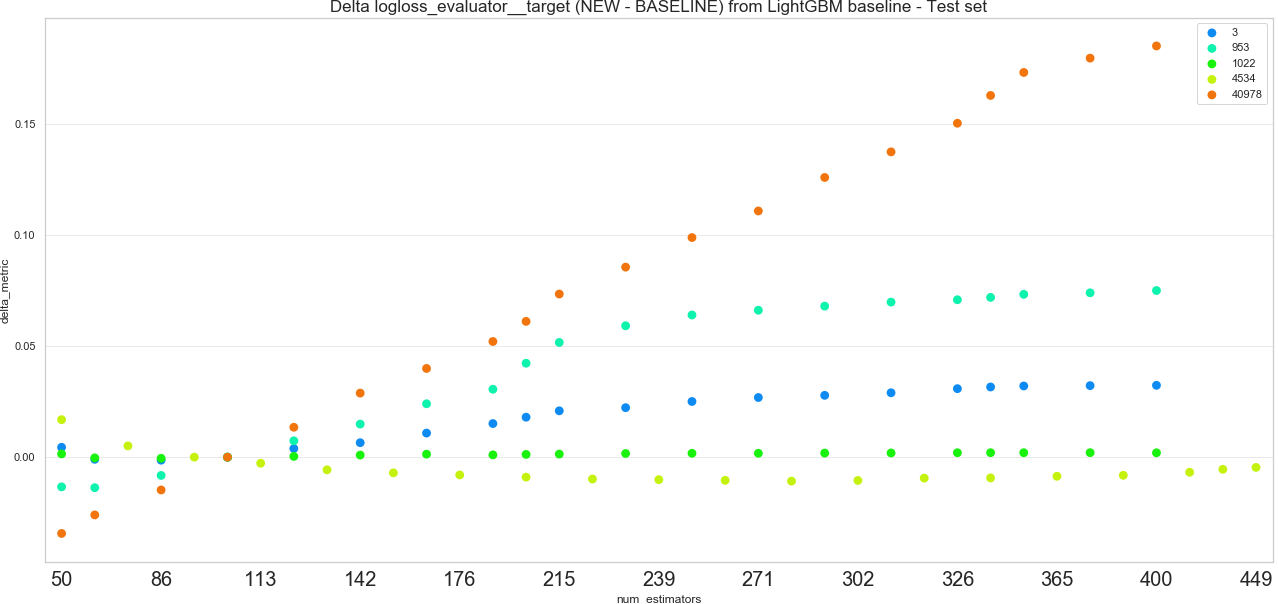
\includegraphics[width=.75\textwidth]{appendix_figures/delta_logloss_cluster2_num_estimators.png}
%     \caption{$\delta_{Logloss}$ plot for $\mathcal{S}(C_2, \eta^{(2)}_{NE}, Logloss)$}
% \end{figure}


% \begin{figure}[H]
%     \centering
%     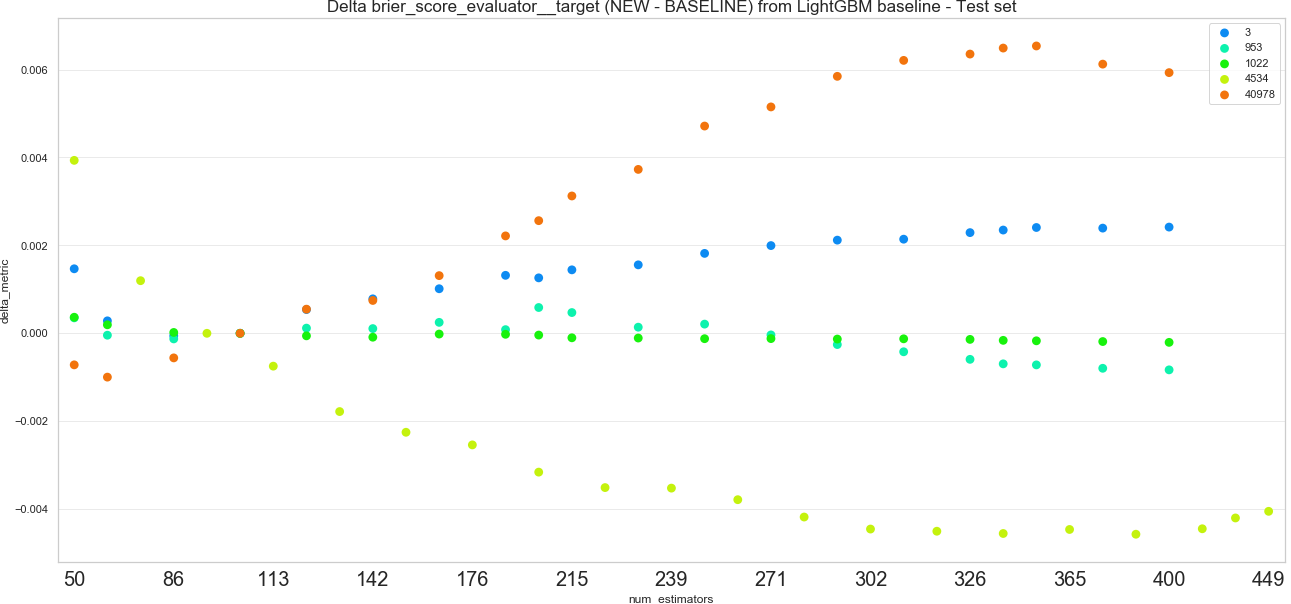
\includegraphics[width=.75\textwidth]{appendix_figures/delta_brier_cluster2_num_estimators.png}
%     \caption{$\delta_{Brier}$ plot for $\mathcal{S}(C_2, \eta^{(2)}_{NE}, Brier)$}
% \end{figure}


% \begin{figure}[H]
%     \centering
%     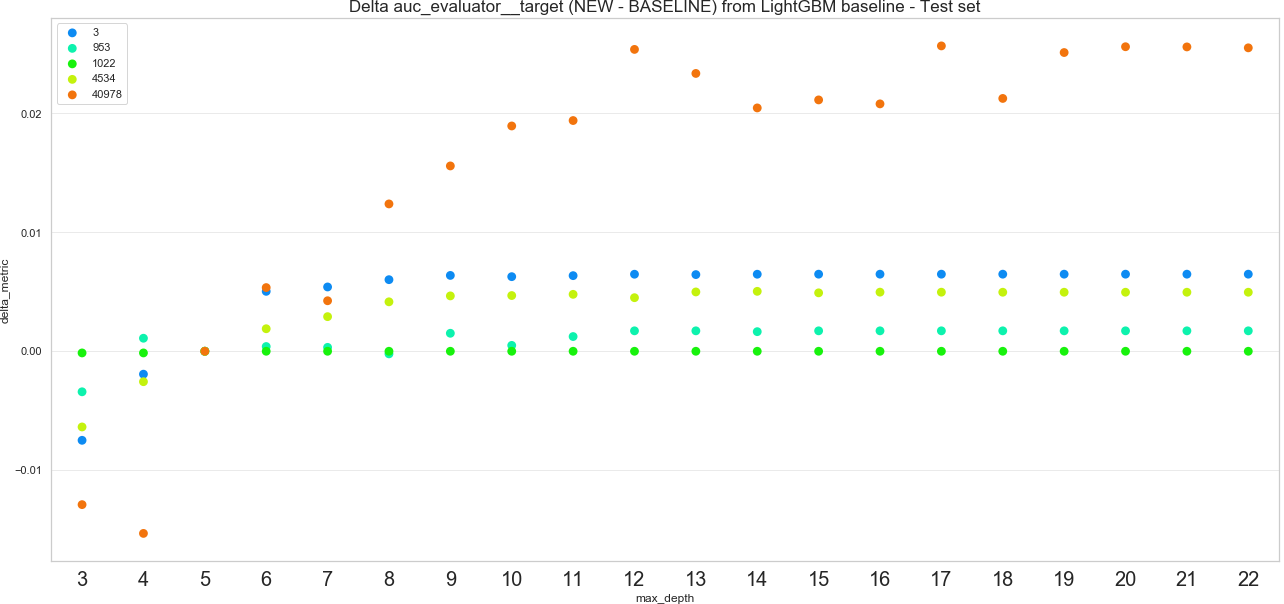
\includegraphics[width=.75\textwidth]{appendix_figures/delta_auc_cluster2_max_depth.png}
%     \caption{$\delta_{AUC}$ plot for $\mathcal{S}(C_2, \eta^{(2)}_{MD}, AUC)$}
% \end{figure}


% \begin{figure}[H]
%     \centering
%     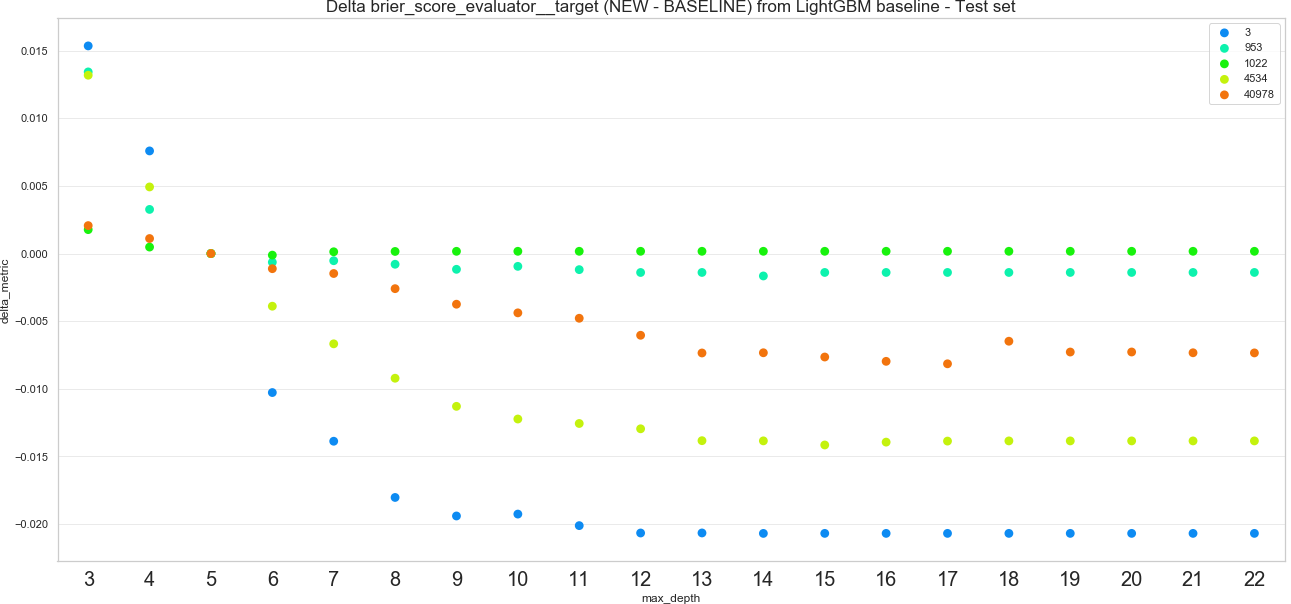
\includegraphics[width=.75\textwidth]{appendix_figures/delta_brier_cluster2_max_depth.png}
%     \caption{$\delta_{Brier}$ plot for $\mathcal{S}(C_2, \eta^{(2)}_{MD}, Brier)$}
% \end{figure}


% \begin{figure}[H]
%     \centering
%     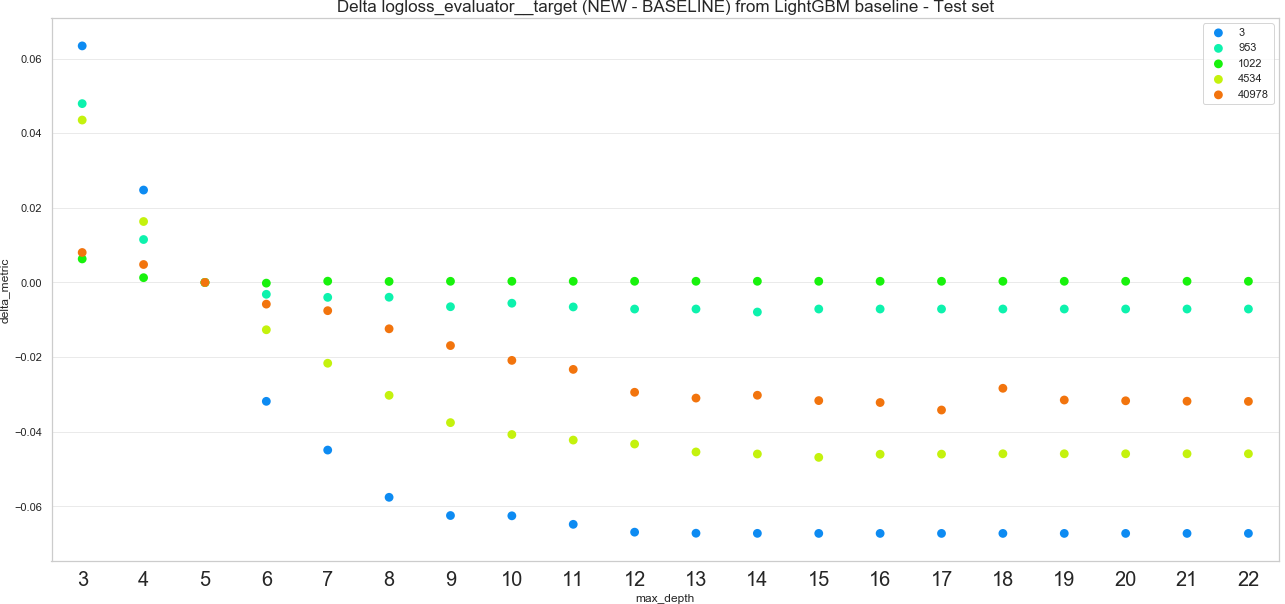
\includegraphics[width=.75\textwidth]{appendix_figures/delta_logloss_cluster2_max_depth.png}
%     \caption{$\delta_{Logloss}$ plot for $\mathcal{S}(C_2, \eta^{(2)}_{MD}, Logloss)$}
% \end{figure}


% \begin{figure}[H]
%     \centering
%     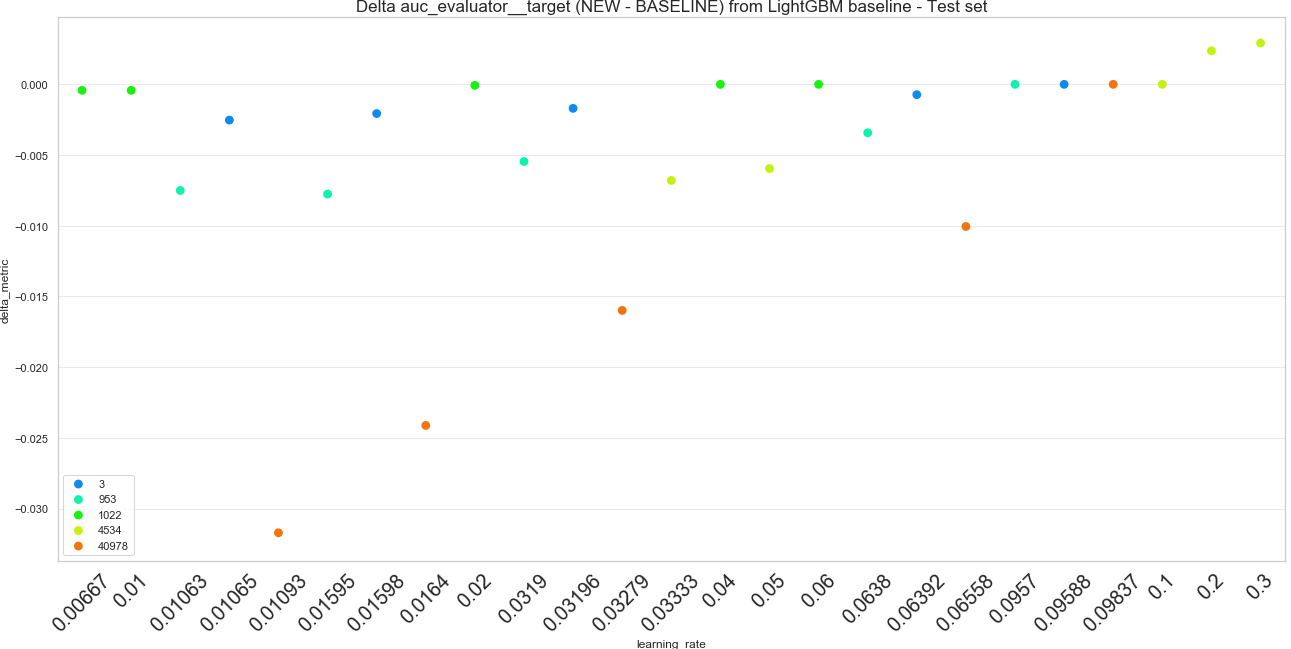
\includegraphics[width=.75\textwidth]{appendix_figures/delta_auc_cluster2_learning_rate.png}
%     \caption{$\delta_{AUC}$ plot for $\mathcal{S}(C_2, \eta^{(2)}_{LR}, AUC)$}
% \end{figure}


% \begin{figure}[H]
%     \centering
%     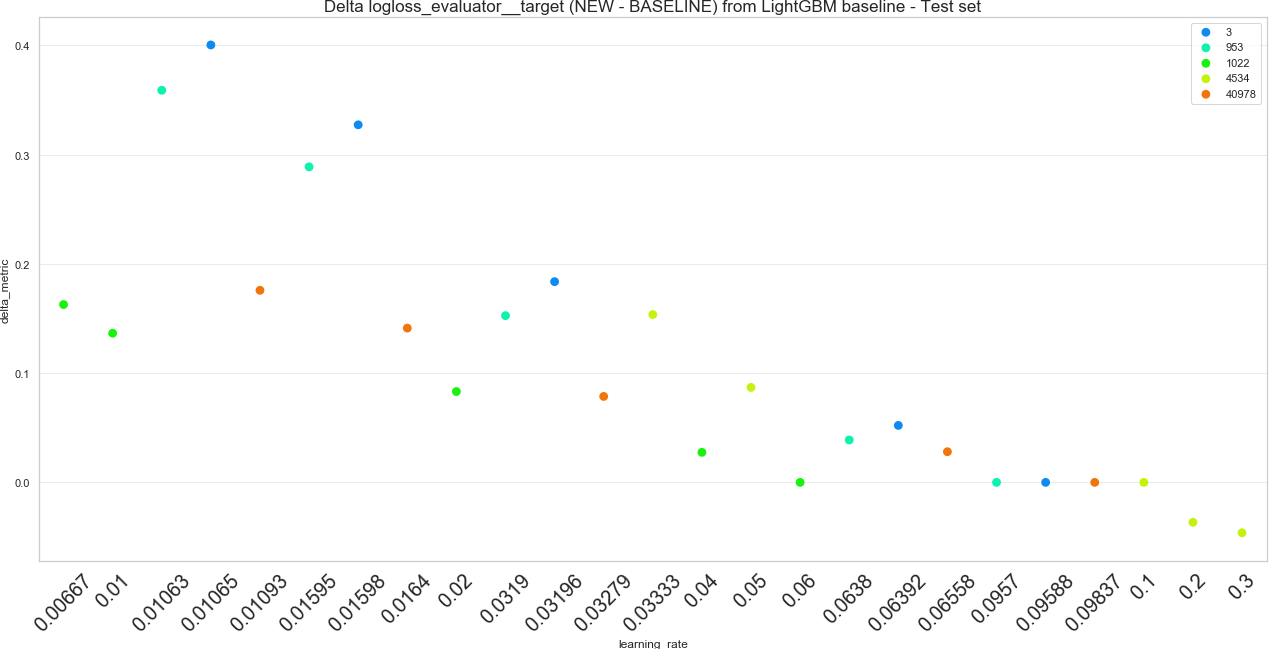
\includegraphics[width=.75\textwidth]{appendix_figures/delta_logloss_cluster2_learning_rate.png}
%     \caption{$\delta_{Logloss}$ plot for $\mathcal{S}(C_2, \eta^{(2)}_{LR}, Logloss)$}
% \end{figure}


% \begin{figure}[H]
%     \centering
%     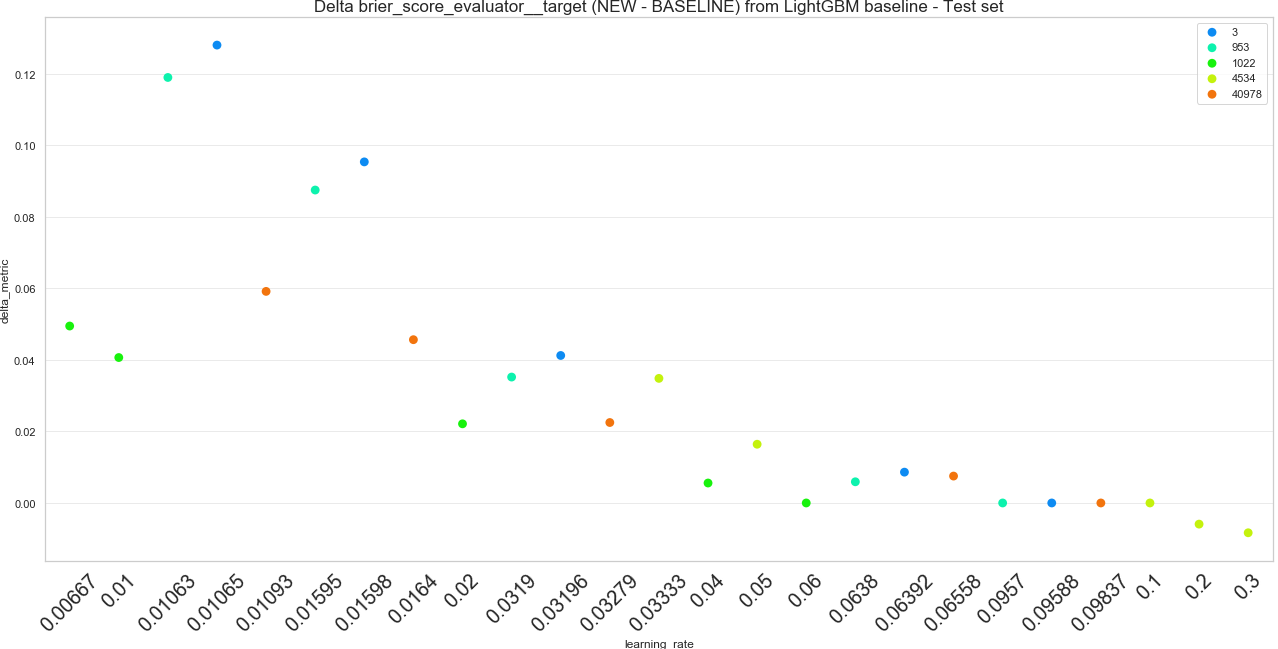
\includegraphics[width=.75\textwidth]{appendix_figures/delta_brier_cluster2_learning_rate.png}
%     \caption{$\delta_{Brier}$ plot for $\mathcal{S}(C_2, \eta^{(2)}_{LR}, Brier)$}
% \end{figure}


% \begin{figure}[H]
%     \centering
%     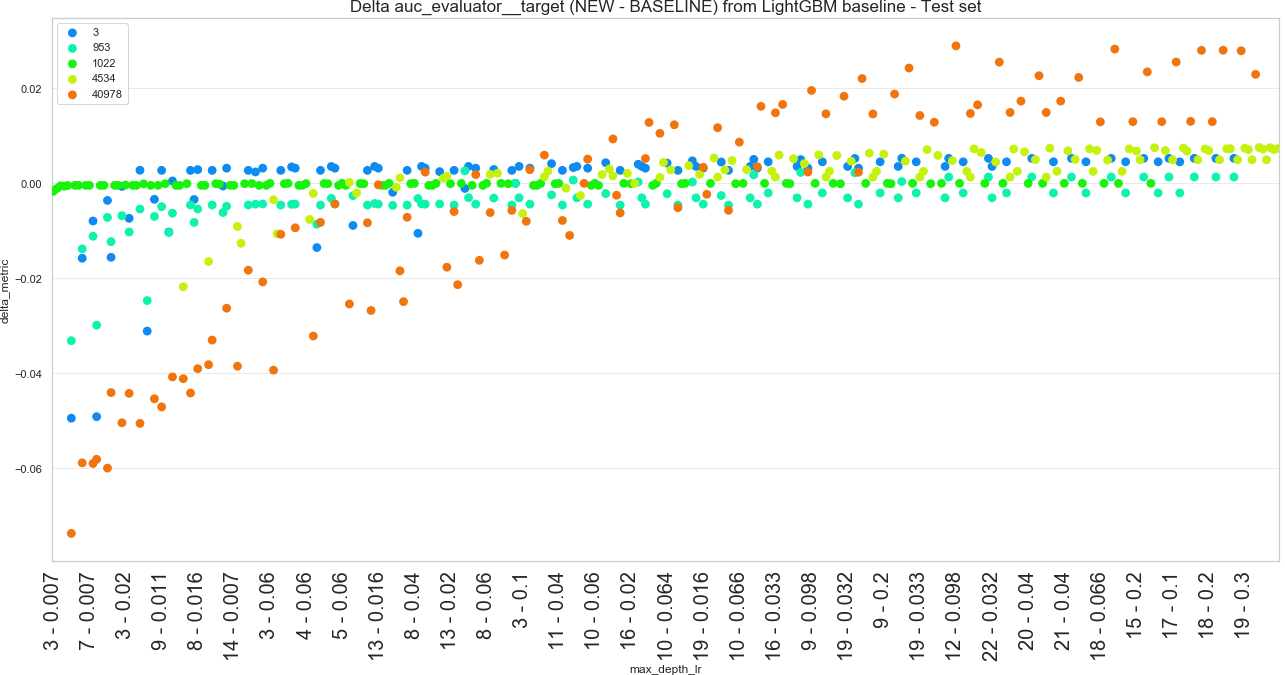
\includegraphics[width=.75\textwidth]{appendix_figures/delta_auc_cluster2_max_depth_lr.png}
%     \caption{$\delta_{AUC}$ plot for $\mathcal{S}(C_2, \eta^{(2)}_{MD, LR}, AUC)$}
% \end{figure}


% \begin{figure}[H]
%     \centering
%     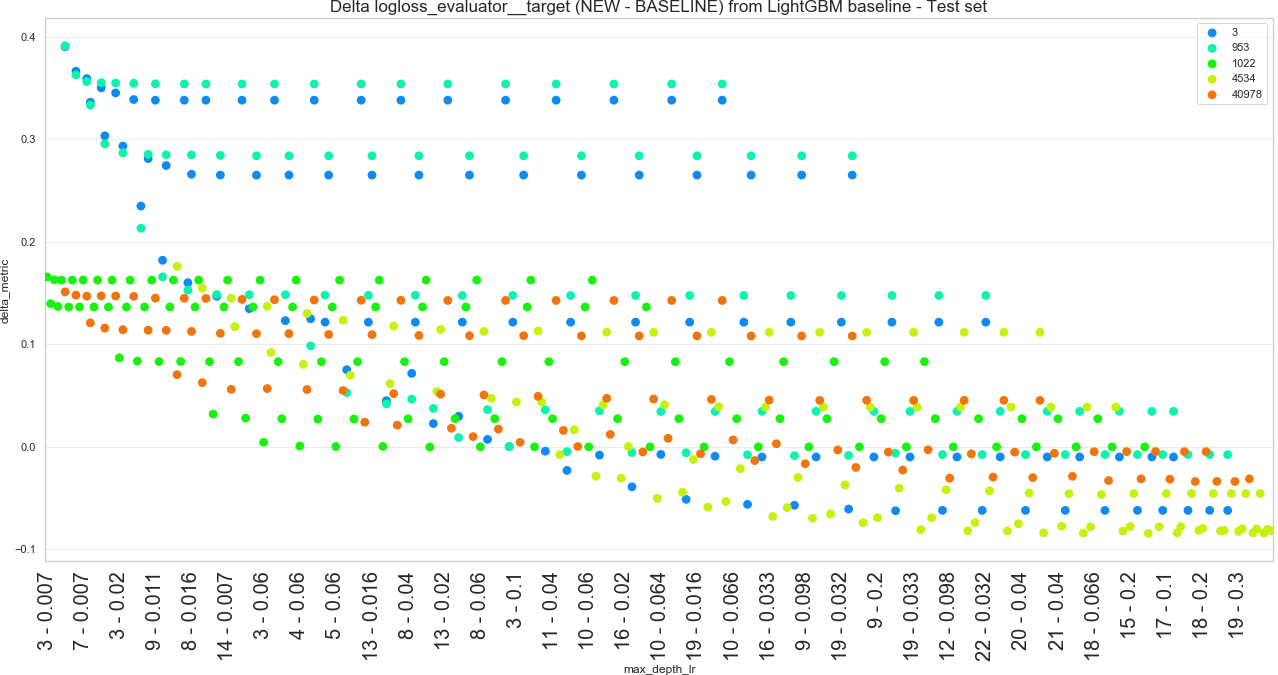
\includegraphics[width=.75\textwidth]{appendix_figures/delta_logloss_cluster2_max_depth_lr.png}
%     \caption{$\delta_{Logloss}$ plot for $\mathcal{S}(C_2, \eta^{(2)}_{MD, LR}, Logloss)$}
% \end{figure}


% \begin{figure}[H]
%     \centering
%     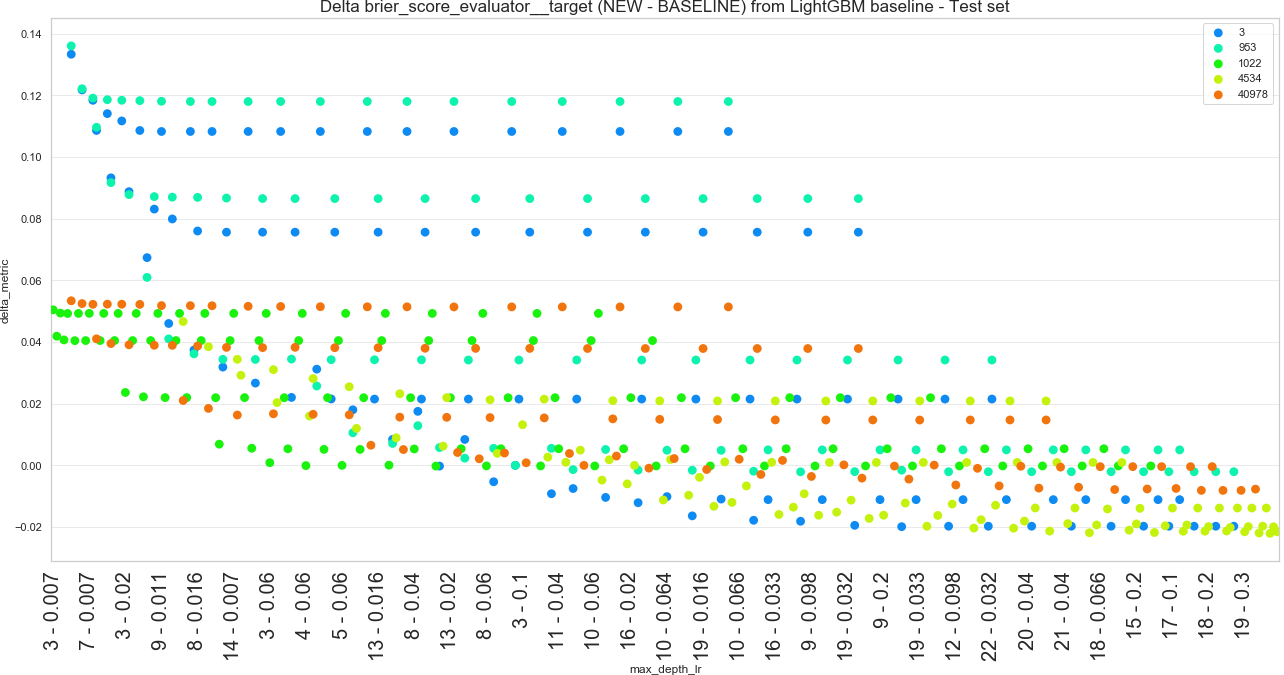
\includegraphics[width=.75\textwidth]{appendix_figures/delta_brier_cluster2_max_depth_lr.png}
%     \caption{$\delta_{Brier}$ plot for $\mathcal{S}(C_2, \eta^{(2)}_{MD, LR}, Brier)$}
% \end{figure}


% \begin{figure}[H]
%     \centering
%     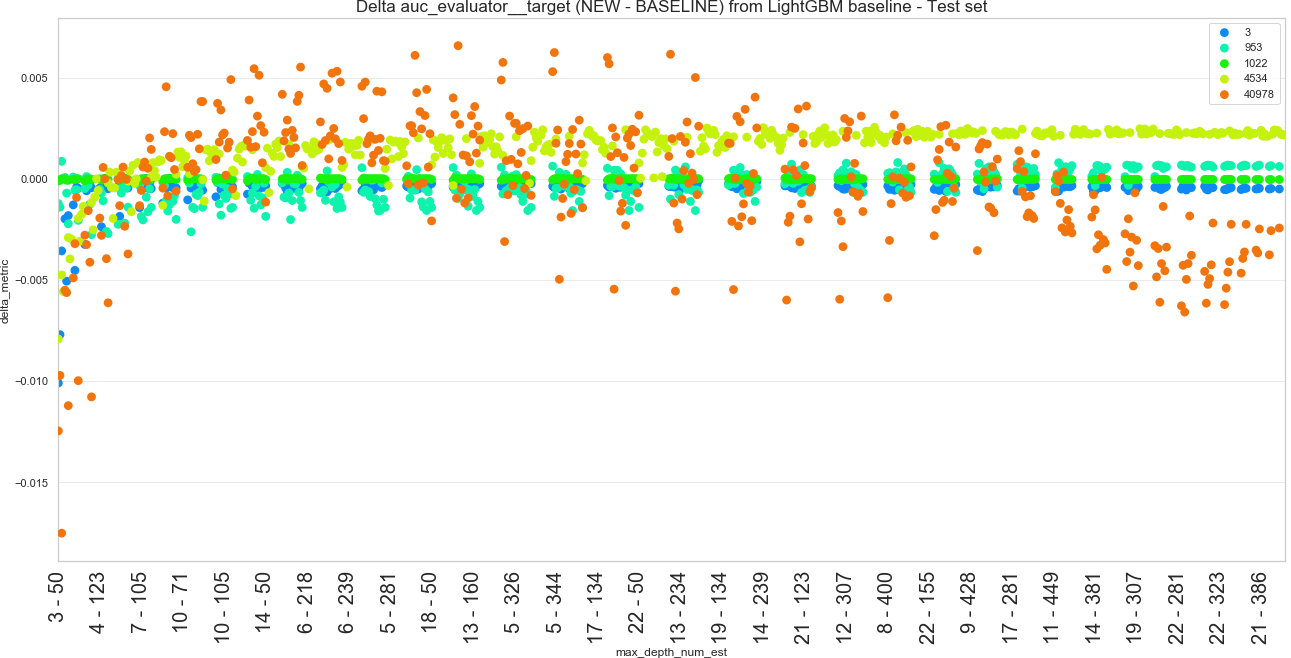
\includegraphics[width=.75\textwidth]{appendix_figures/delta_auc_cluster2_max_depth_num_est.png}
%     \caption{$\delta_{AUC}$ plot for $\mathcal{S}(C_2, \eta^{(2)}_{MD, NE}, AUC)$}
% \end{figure}


% \begin{figure}[H]
%     \centering
%     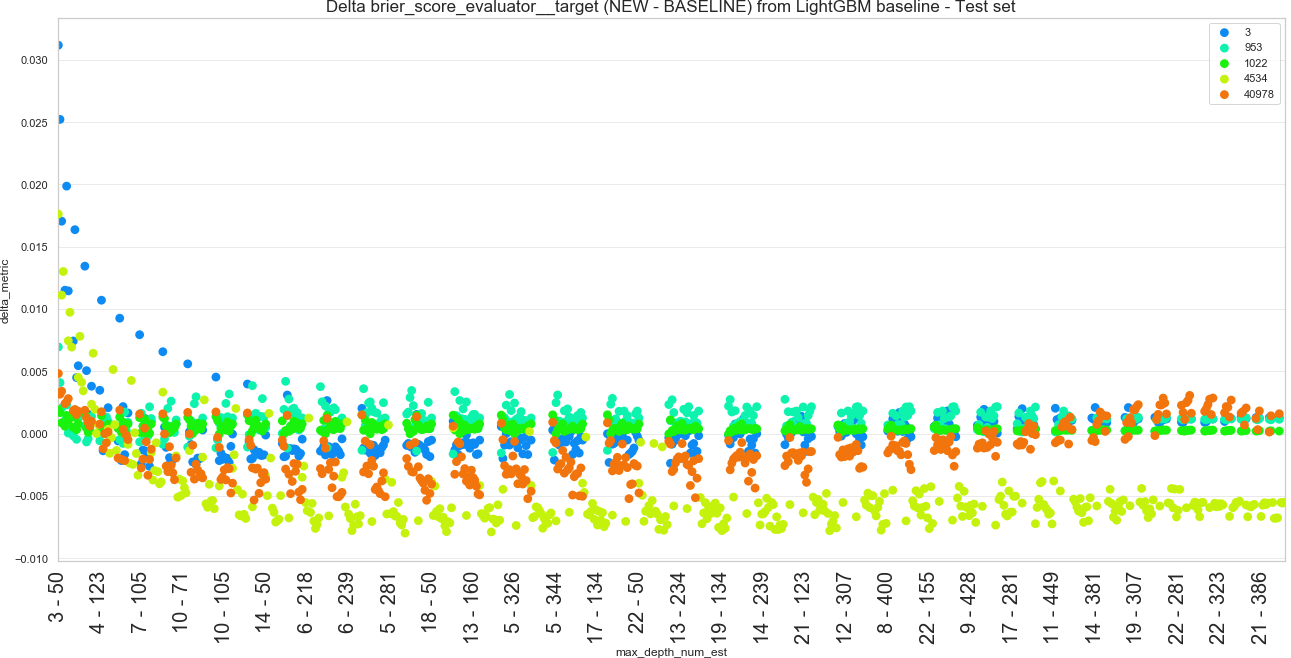
\includegraphics[width=.75\textwidth]{appendix_figures/delta_brier_cluster2_max_depth_num_est.png}
%     \caption{$\delta_{Brier}$ plot for $\mathcal{S}(C_2, \eta^{(2)}_{MD, NE}, Brier)$}
% \end{figure}


% \begin{figure}[H]
%     \centering
%     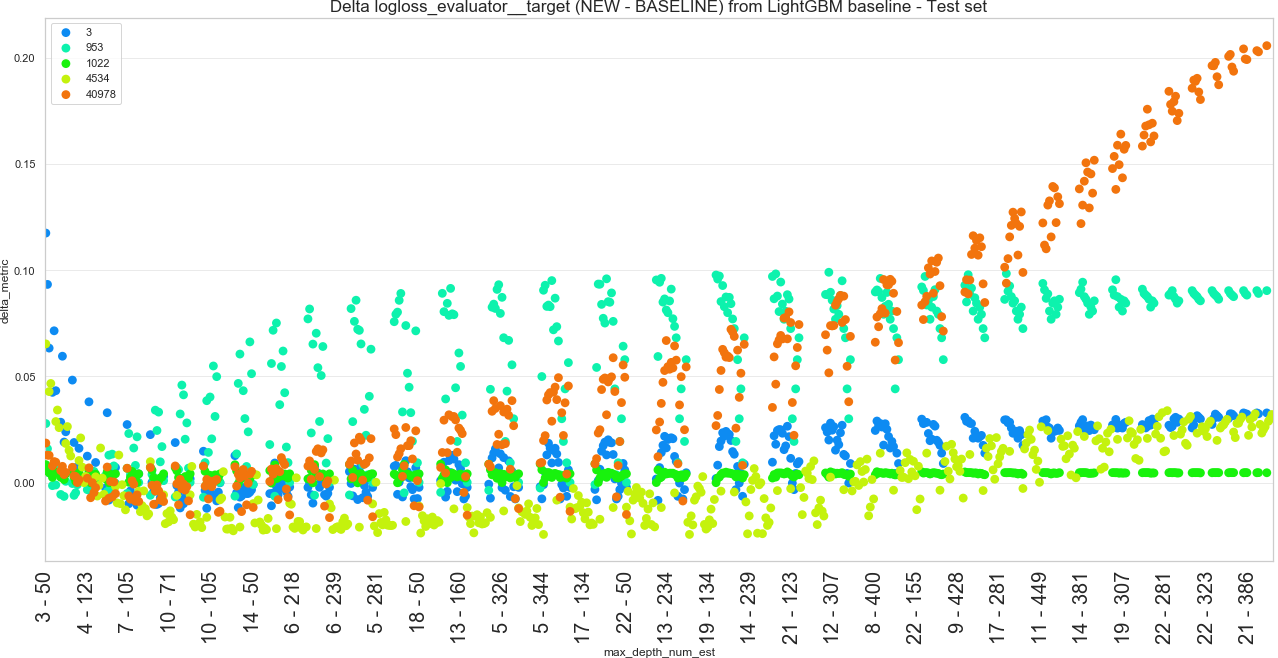
\includegraphics[width=.75\textwidth]{appendix_figures/delta_logloss_cluster2_max_depth_num_est.png}
%     \caption{$\delta_{Logloss}$ plot for $\mathcal{S}(C_2, \eta^{(2)}_{MD, NE}, Logloss)$}
% \end{figure}


% \begin{figure}[H]
%     \centering
%     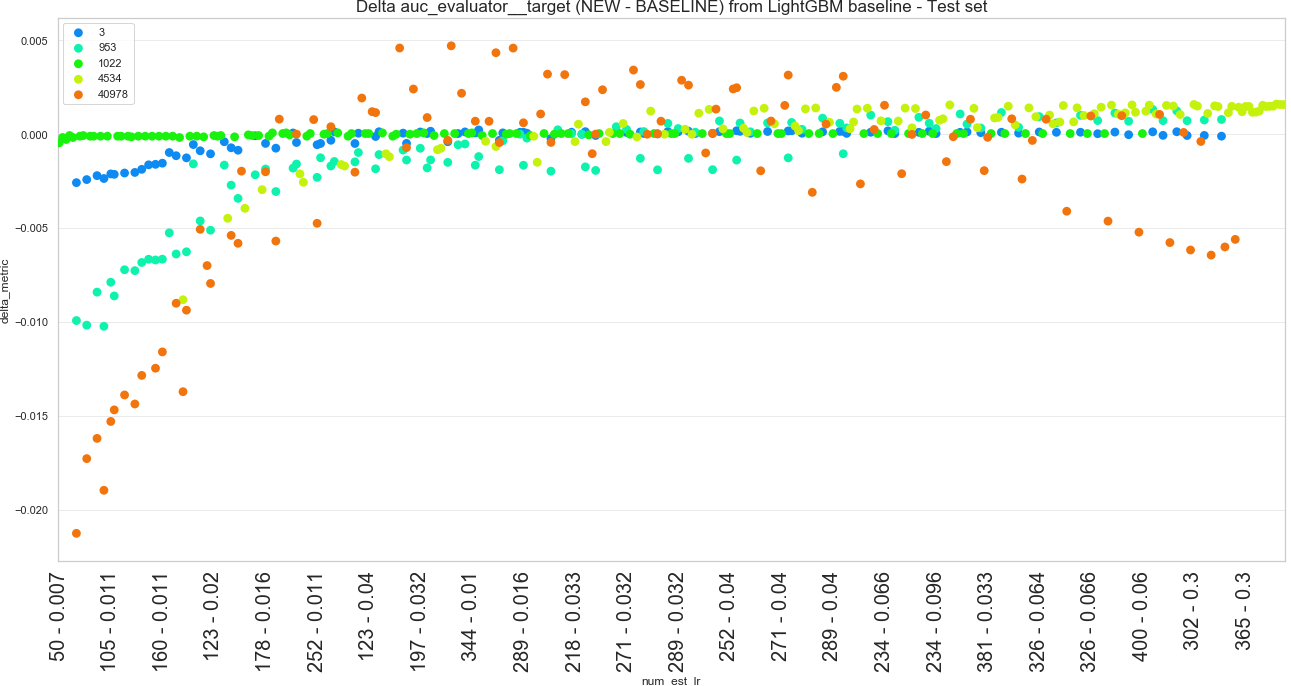
\includegraphics[width=.75\textwidth]{appendix_figures/delta_auc_cluster2_num_est_lr.png}
%     \caption{$\delta_{AUC}$ plot for $\mathcal{S}(C_2, \eta^{(2)}_{LR, NE}, AUC)$}
% \end{figure}


% \begin{figure}[H]
%     \centering
%     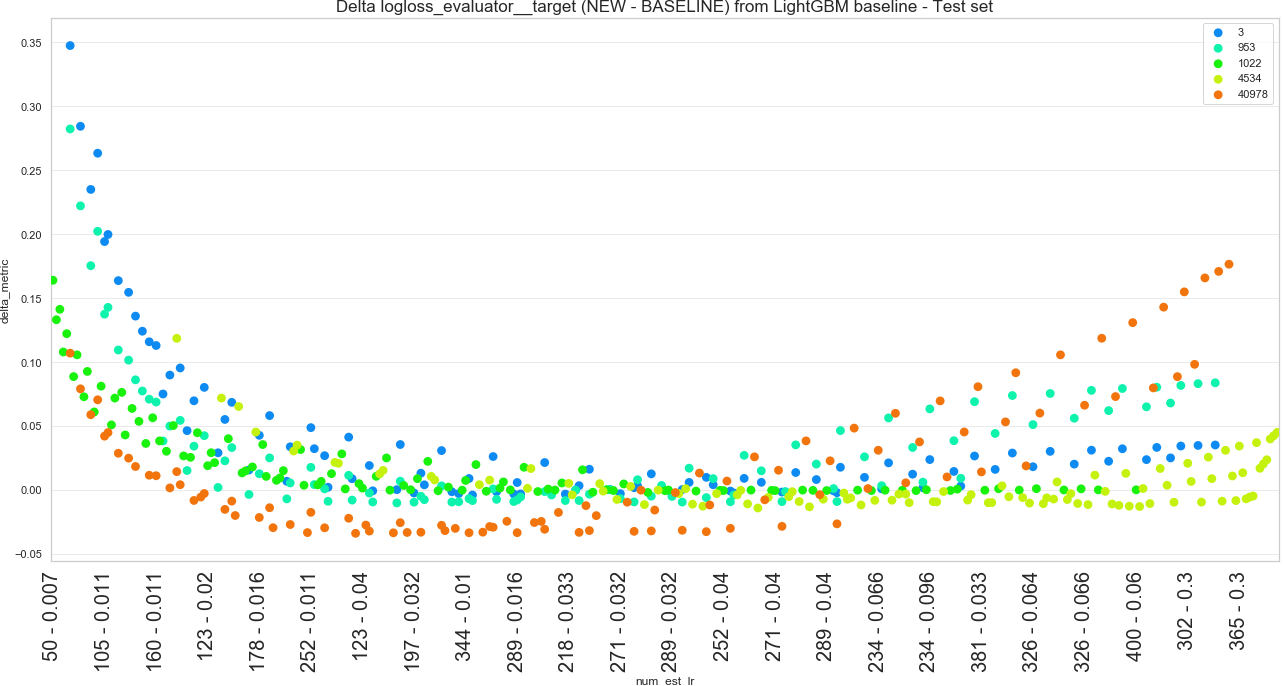
\includegraphics[width=.75\textwidth]{appendix_figures/delta_logloss_cluster2_num_est_lr.png}
%     \caption{$\delta_{Logloss}$ plot for $\mathcal{S}(C_2, \eta^{(2)}_{LR, NE}, Logloss)$}
% \end{figure}


% \begin{figure}[H]
%     \centering
%     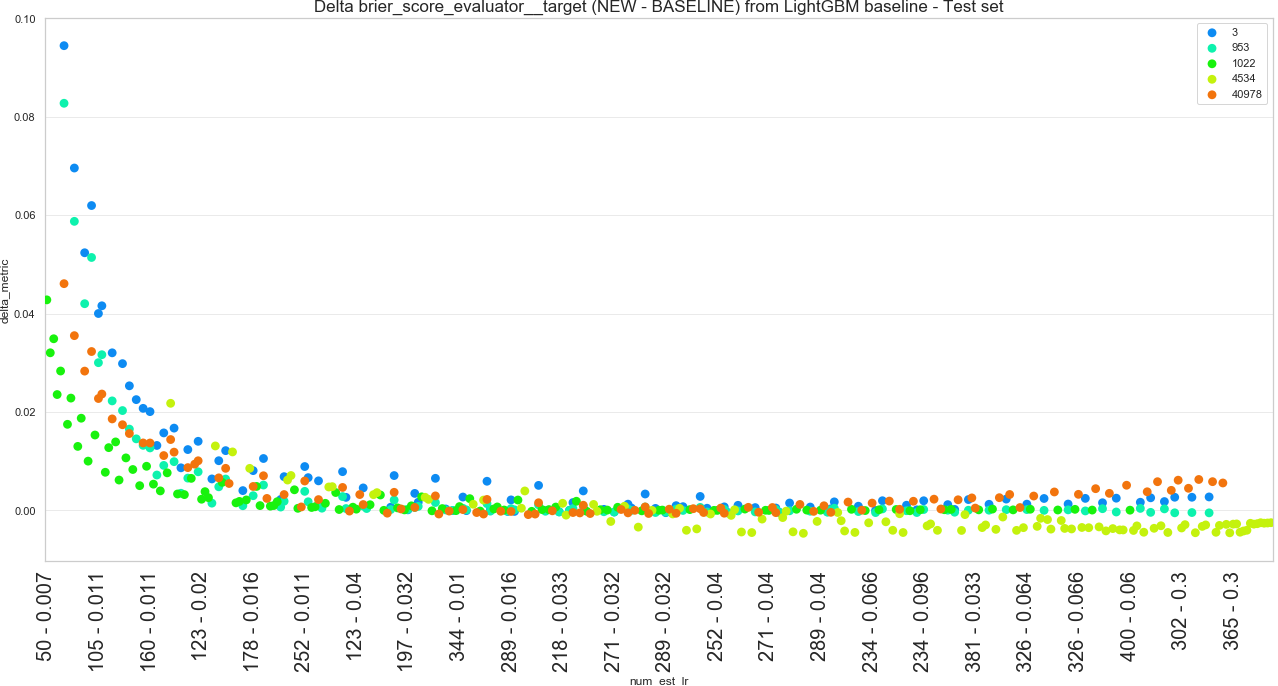
\includegraphics[width=.75\textwidth]{appendix_figures/delta_brier_cluster2_num_est_lr.png}
%     \caption{$\delta_{Brier}$ plot for $\mathcal{S}(C_2, \eta^{(2)}_{LR, NE}, Brier)$}
% \end{figure}


% \begin{figure}[H]
%     \centering
%     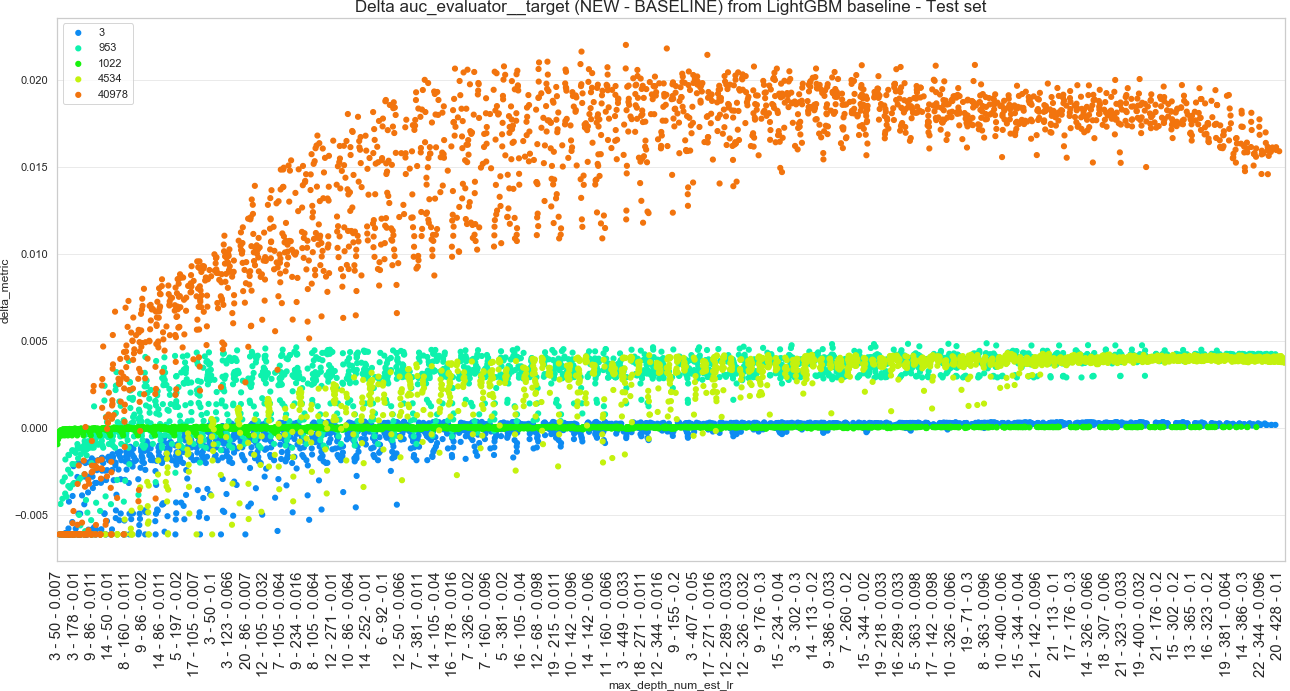
\includegraphics[width=.75\textwidth]{appendix_figures/delta_auc_cluster2_max_depth_num_est_lr.png}
%     \caption{$\delta_{AUC}$ plot for $\mathcal{S}(C_2, \eta^{(2)}_{NE, MD, LR}, AUC)$}
% \end{figure}


% \begin{figure}[H]
%     \centering
%     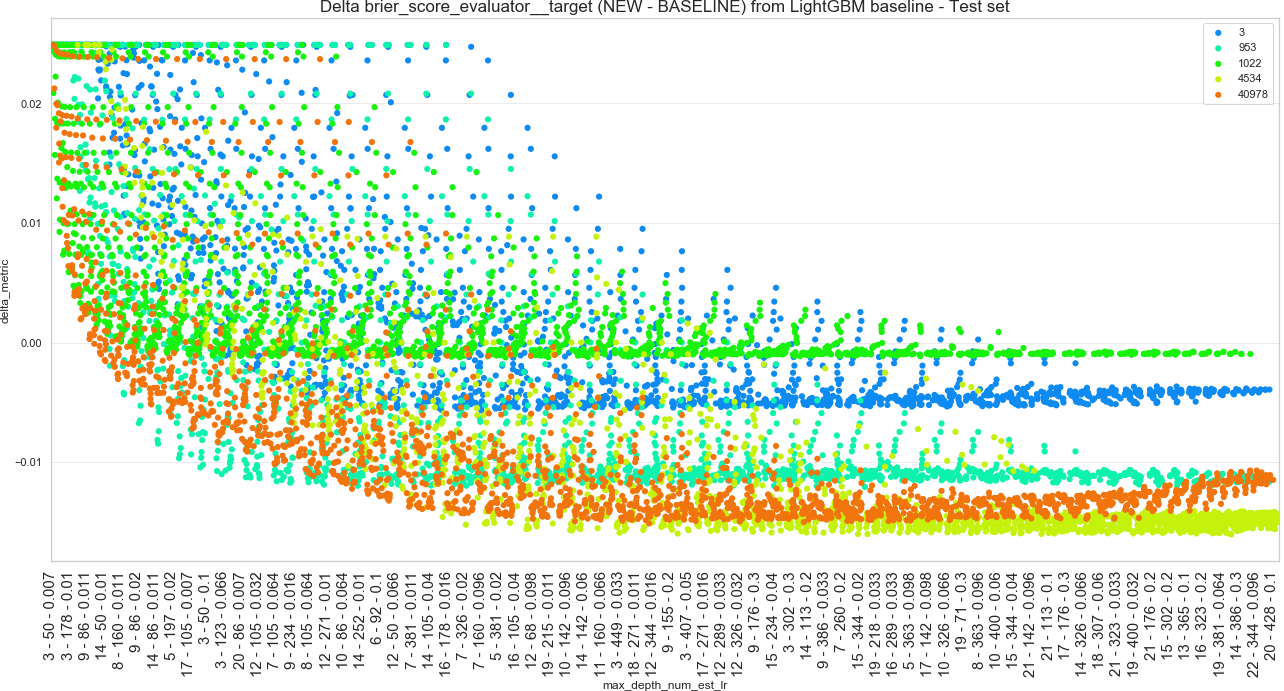
\includegraphics[width=.75\textwidth]{appendix_figures/delta_brier_cluster2_max_depth_num_est_lr.png}
%     \caption{$\delta_{Brier}$ plot for $\mathcal{S}(C_2, \eta^{(2)}_{NE, MD, LR}, Brier)$}
% \end{figure}


% \begin{figure}[H]
%     \centering
%     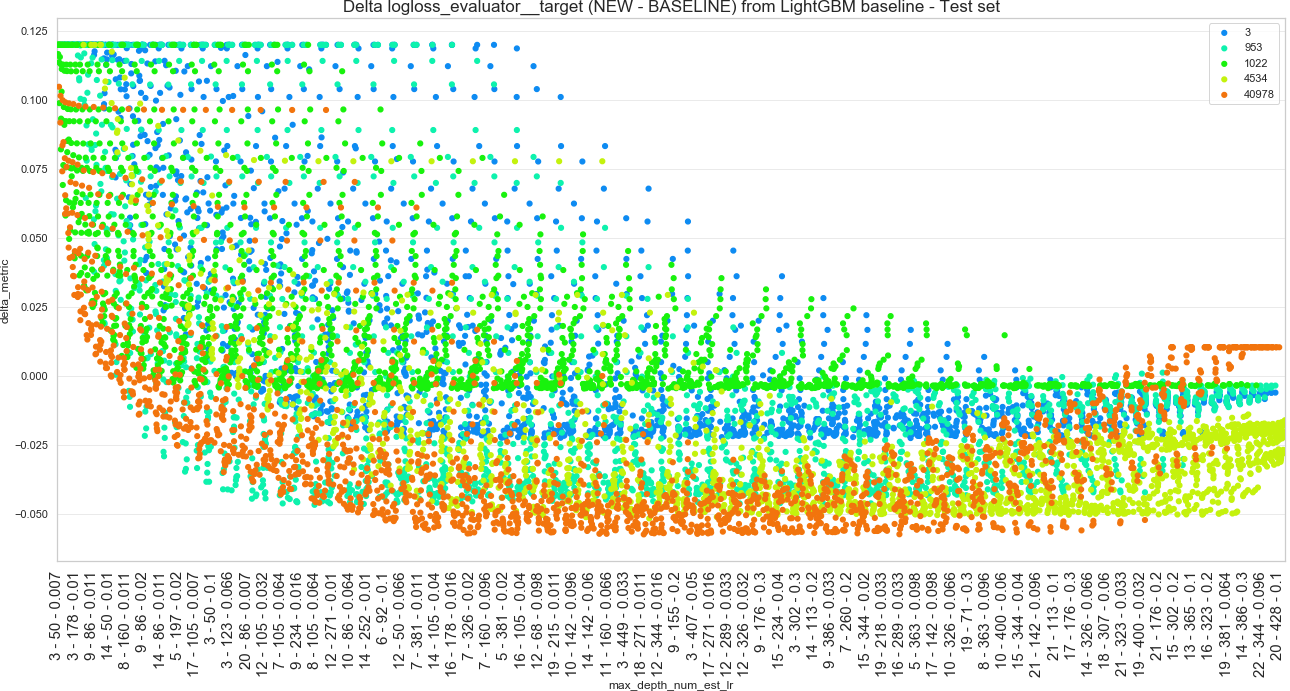
\includegraphics[width=.75\textwidth]{appendix_figures/delta_logloss_cluster2_max_depth_num_est_lr.png}
%     \caption{$\delta_{Logloss}$ plot for $\mathcal{S}(C_2, \eta^{(2)}_{NE, MD, LR}, Logloss)$}
% \end{figure}


% \begin{figure}[H]
%     \centering
%     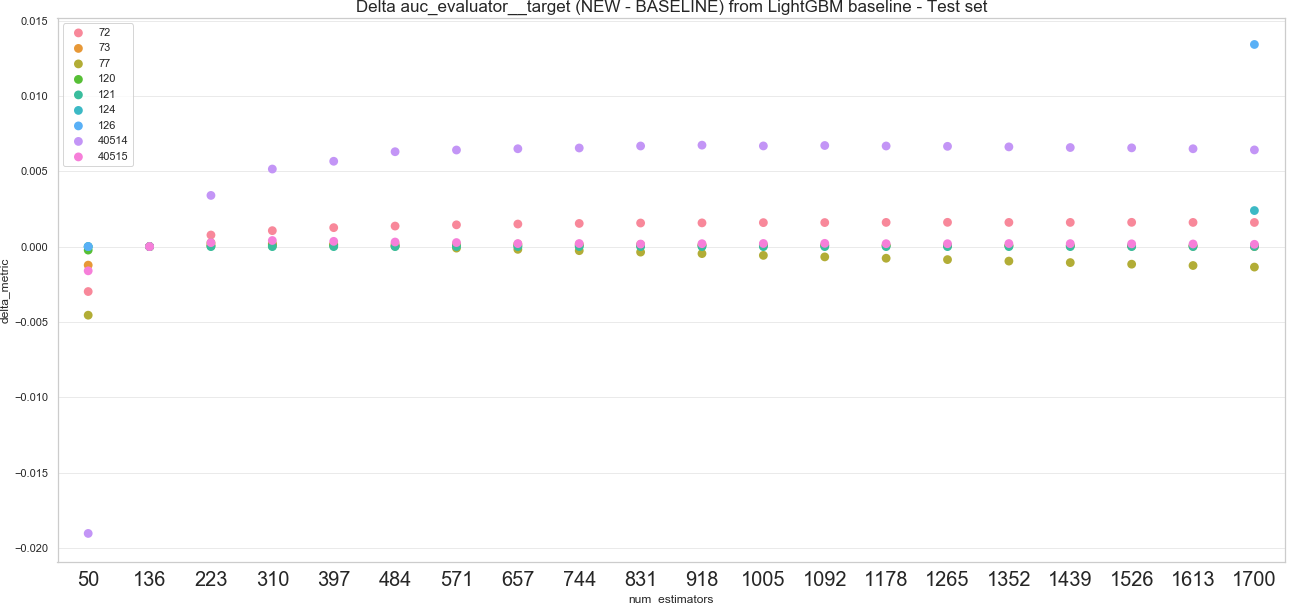
\includegraphics[width=.75\textwidth]{appendix_figures/delta_auc_cluster3_num_estimators.png}
%     \caption{$\delta_{AUC}$ plot for $\mathcal{S}(C_3, \eta^{(3)}_{NE}, AUC)$}
% \end{figure}


% \begin{figure}[H]
%     \centering
%     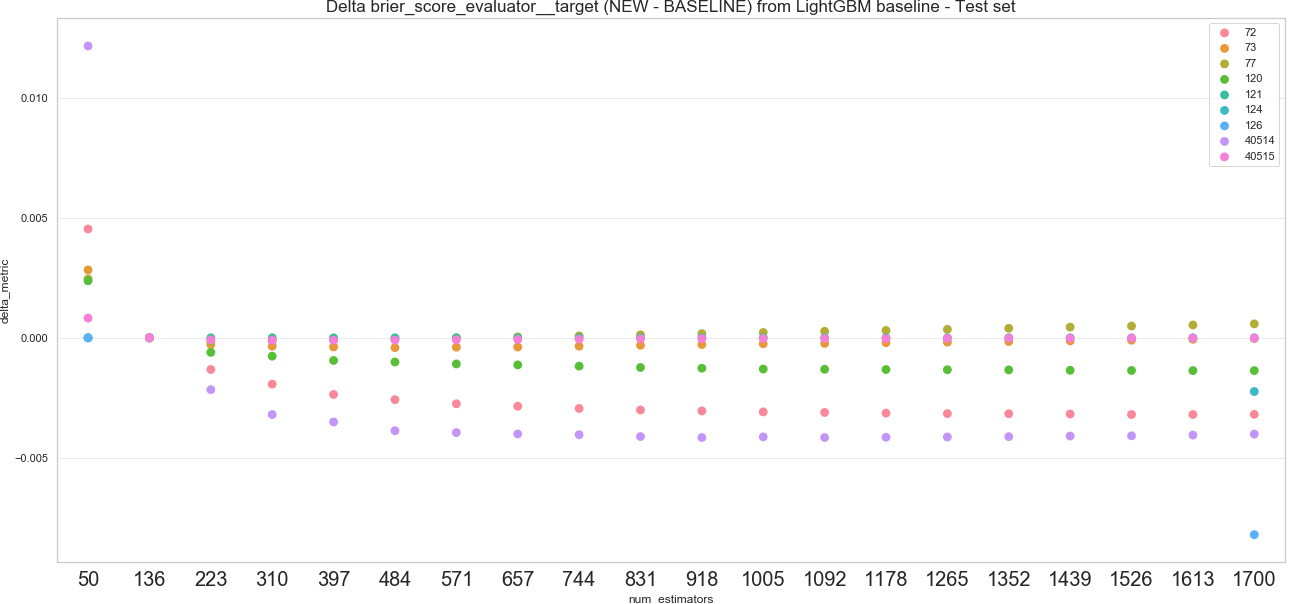
\includegraphics[width=.75\textwidth]{appendix_figures/delta_brier_cluster3_num_estimators.png}
%     \caption{$\delta_{Brier}$ plot for $\mathcal{S}(C_3, \eta^{(3)}_{NE}, Brier)$}
% \end{figure}


% \begin{figure}[H]
%     \centering
%     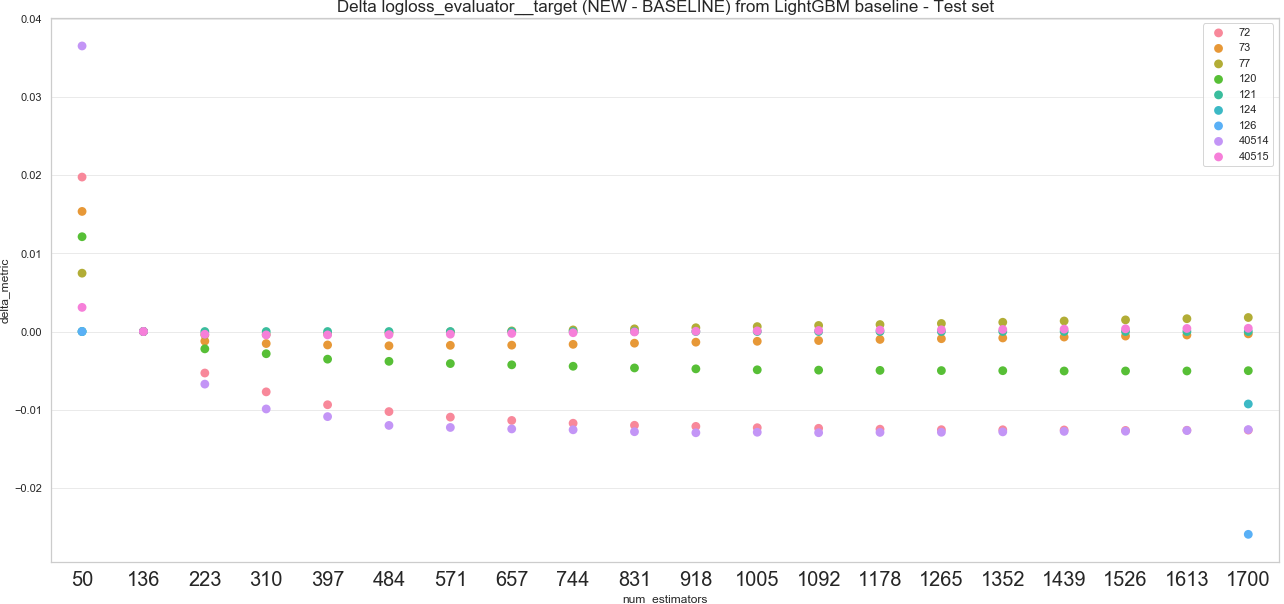
\includegraphics[width=.75\textwidth]{appendix_figures/delta_logloss_cluster3_num_estimators.png}
%     \caption{$\delta_{Logloss}$ plot for $\mathcal{S}(C_3, \eta^{(3)}_{NE}, Logloss)$}
% \end{figure}


% \begin{figure}[H]
%     \centering
%     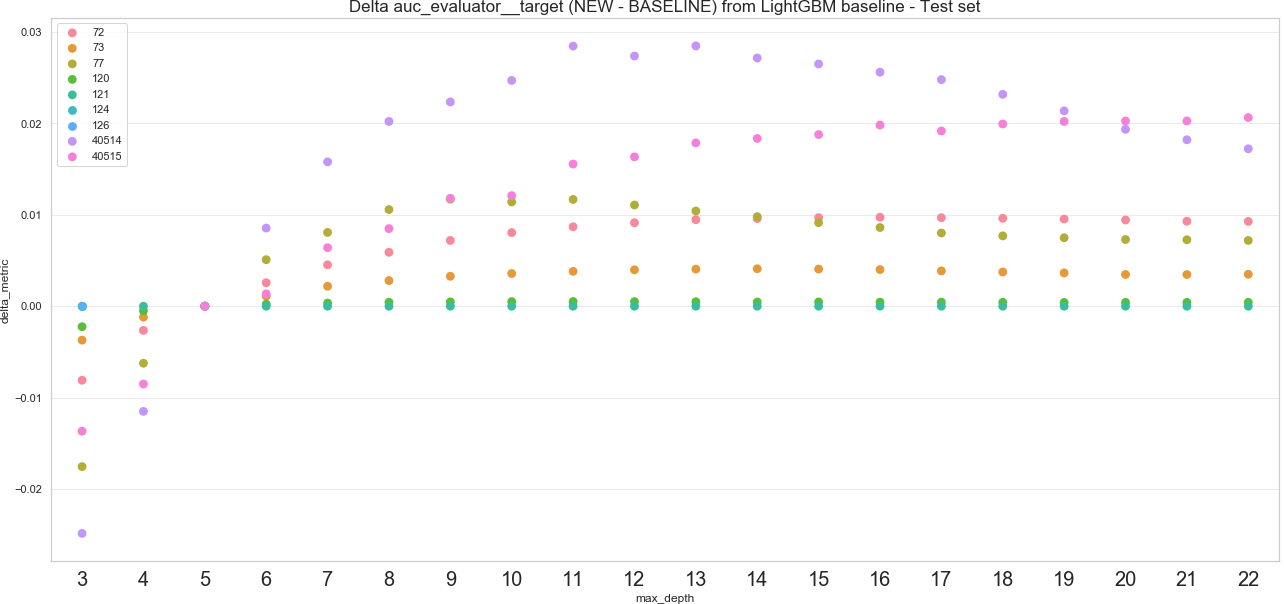
\includegraphics[width=.75\textwidth]{appendix_figures/delta_auc_cluster3_max_depth.png}
%     \caption{$\delta_{AUC}$ plot for $\mathcal{S}(C_3, \eta^{(3)}_{MD}, AUC)$}
% \end{figure}


% \begin{figure}[H]
%     \centering
%     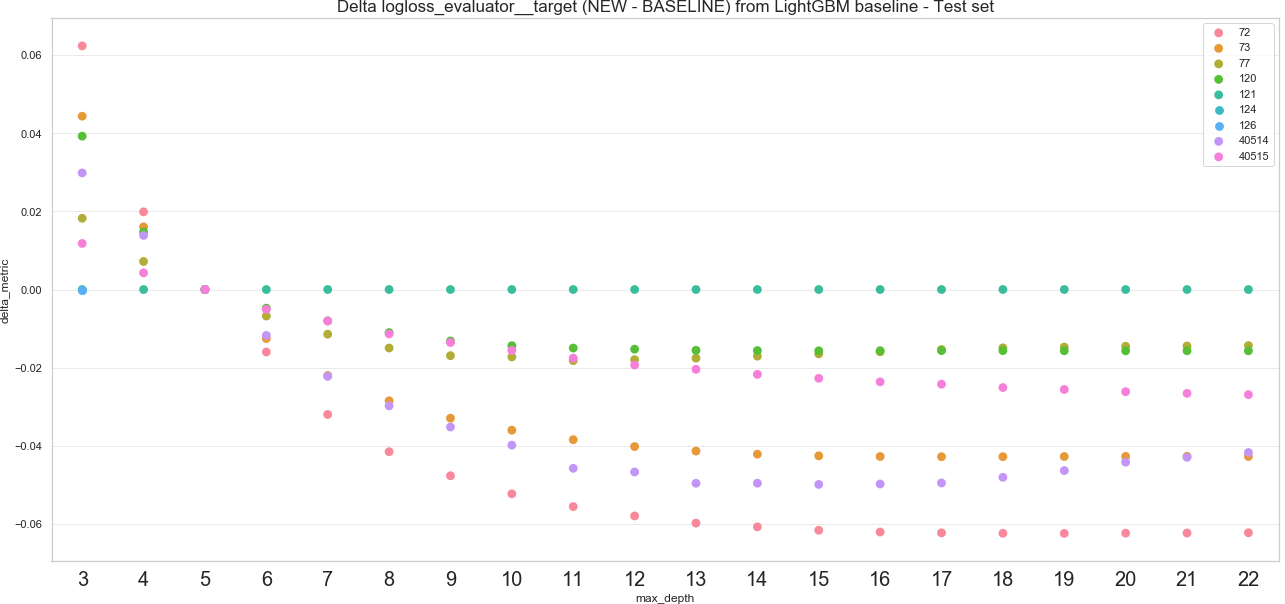
\includegraphics[width=.75\textwidth]{appendix_figures/delta_logloss_cluster3_max_depth.png}
%     \caption{$\delta_{Logloss}$ plot for $\mathcal{S}(C_3, \eta^{(3)}_{MD}, Logloss)$}
% \end{figure}


% \begin{figure}[H]
%     \centering
%     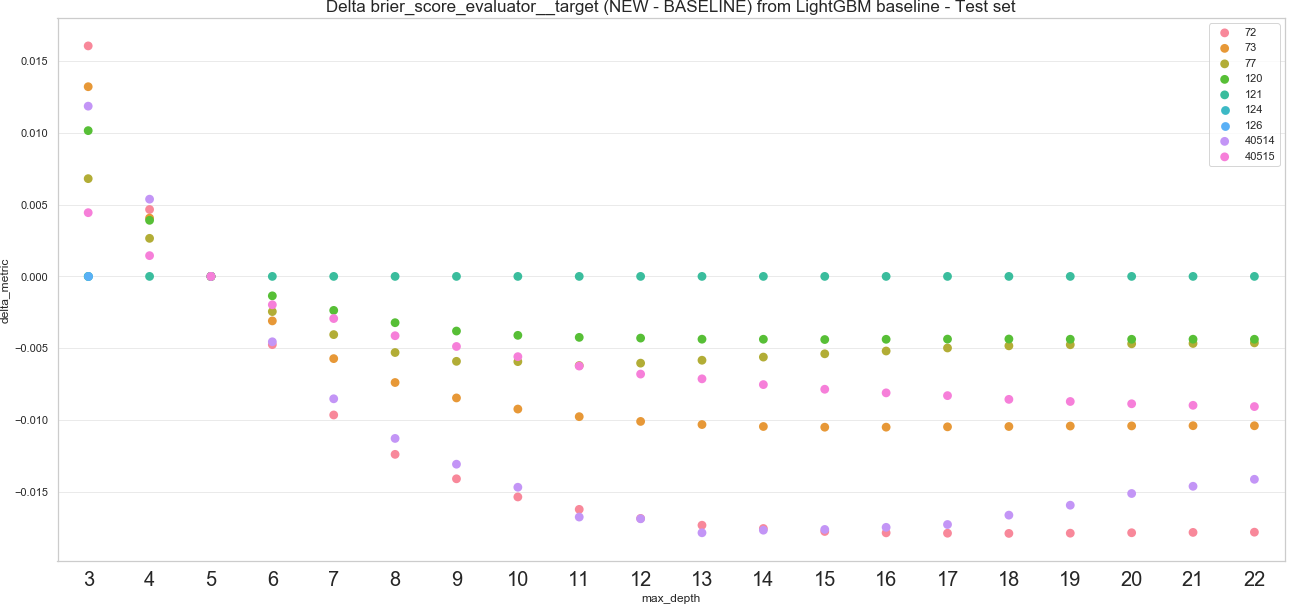
\includegraphics[width=.75\textwidth]{appendix_figures/delta_brier_cluster3_max_depth.png}
%     \caption{$\delta_{Brier}$ plot for $\mathcal{S}(C_3, \eta^{(3)}_{MD}, Brier)$}
% \end{figure}


% \begin{figure}[H]
%     \centering
%     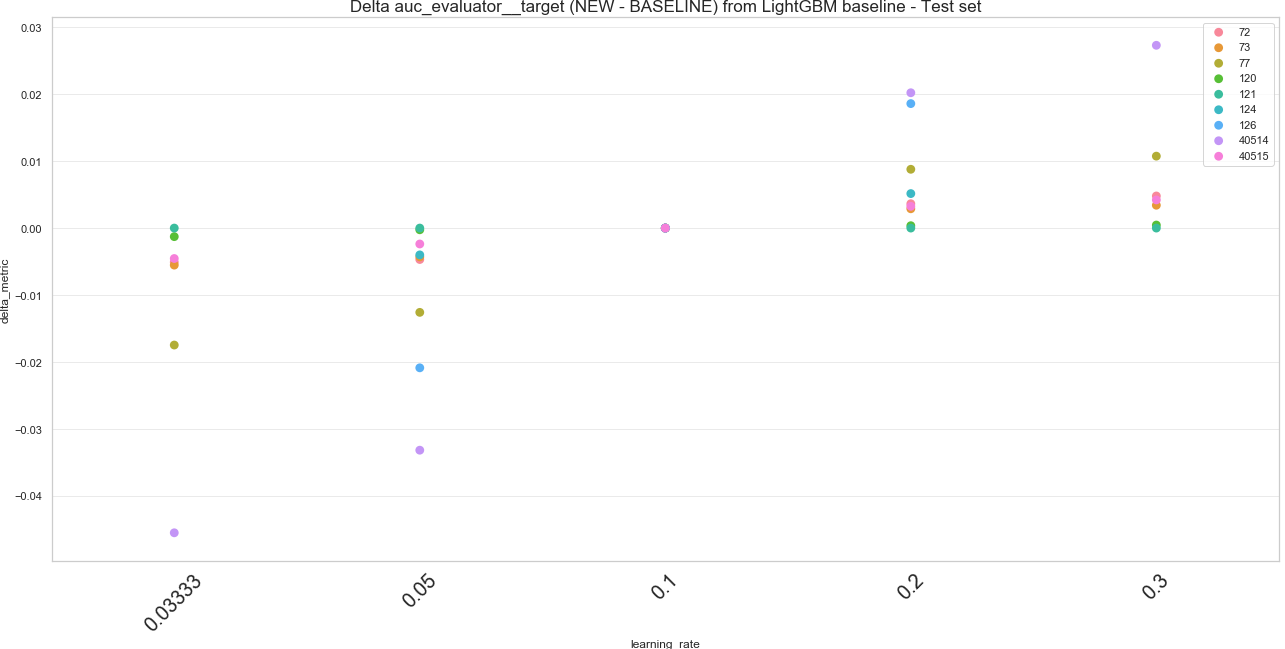
\includegraphics[width=.75\textwidth]{appendix_figures/delta_auc_cluster3_learning_rate.png}
%     \caption{$\delta_{AUC}$ plot for $\mathcal{S}(C_3, \eta^{(3)}_{LR}, AUC)$}
% \end{figure}


% \begin{figure}[H]
%     \centering
%     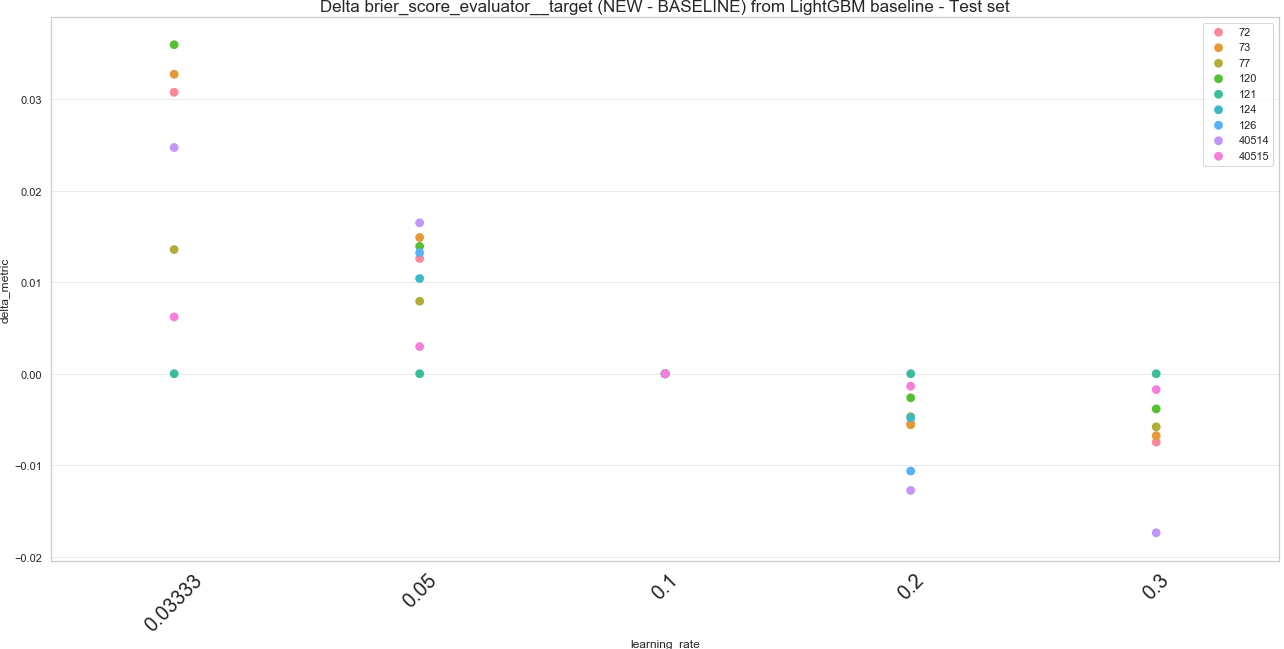
\includegraphics[width=.75\textwidth]{appendix_figures/delta_brier_cluster3_learning_rate.png}
%     \caption{$\delta_{Brier}$ plot for $\mathcal{S}(C_3, \eta^{(3)}_{LR}, Brier)$}
% \end{figure}


% \begin{figure}[H]
%     \centering
%     \includegraphics[width=.75\textwidth]{appendix_figures/delta_logloss_cluster3_learning_rate.png}
%     \caption{$\delta_{Logloss}$ plot for $\mathcal{S}(C_3, \eta^{(3)}_{LR}, Logloss)$}
% \end{figure}


% \begin{figure}[H]
%     \centering
%     \includegraphics[width=.75\textwidth]{appendix_figures/delta_auc_cluster3_max_depth_lr.png}
%     \caption{$\delta_{AUC}$ plot for $\mathcal{S}(C_3, \eta^{(3)}_{MD, LR}, AUC)$}
% \end{figure}


% \begin{figure}[H]
%     \centering
%     \includegraphics[width=.75\textwidth]{appendix_figures/delta_logloss_cluster3_max_depth_lr.png}
%     \caption{$\delta_{Logloss}$ plot for $\mathcal{S}(C_3, \eta^{(3)}_{MD, LR}, Logloss)$}
% \end{figure}


% \begin{figure}[H]
%     \centering
%     \includegraphics[width=.75\textwidth]{appendix_figures/delta_brier_cluster3_max_depth_lr.png}
%     \caption{$\delta_{Brier}$ plot for $\mathcal{S}(C_3, \eta^{(3)}_{MD, LR}, Brier)$}
% \end{figure}


% \begin{figure}[H]
%     \centering
%     \includegraphics[width=.75\textwidth]{appendix_figures/delta_auc_cluster3_max_depth_num_est.png}
%     \caption{$\delta_{AUC}$ plot for $\mathcal{S}(C_3, \eta^{(3)}_{MD, NE}, AUC)$}
% \end{figure}


% \begin{figure}[H]
%     \centering
%     \includegraphics[width=.75\textwidth]{appendix_figures/delta_logloss_cluster3_max_depth_num_est.png}
%     \caption{$\delta_{Logloss}$ plot for $\mathcal{S}(C_3, \eta^{(3)}_{MD, NE}, Logloss)$}
% \end{figure}


% \begin{figure}[H]
%     \centering
%     \includegraphics[width=.75\textwidth]{appendix_figures/delta_brier_cluster3_max_depth_num_est.png}
%     \caption{$\delta_{Brier}$ plot for $\mathcal{S}(C_3, \eta^{(3)}_{MD, NE}, Brier)$}
% \end{figure}


% \begin{figure}[H]
%     \centering
%     \includegraphics[width=.75\textwidth]{appendix_figures/delta_auc_cluster3_num_est_lr.png}
%     \caption{$\delta_{AUC}$ plot for $\mathcal{S}(C_3, \eta^{(3)}_{LR, NE}, AUC)$}
% \end{figure}


% \begin{figure}[H]
%     \centering
%     \includegraphics[width=.75\textwidth]{appendix_figures/delta_brier_cluster3_num_est_lr.png}
%     \caption{$\delta_{Brier}$ plot for $\mathcal{S}(C_3, \eta^{(3)}_{LR, NE}, Brier)$}
% \end{figure}


% \begin{figure}[H]
%     \centering
%     \includegraphics[width=.75\textwidth]{appendix_figures/delta_logloss_cluster3_num_est_lr.png}
%     \caption{$\delta_{Logloss}$ plot for $\mathcal{S}(C_3, \eta^{(3)}_{LR, NE}, Logloss)$}
% \end{figure}


% \begin{figure}[H]
%     \centering
%     \includegraphics[width=.75\textwidth]{appendix_figures/delta_auc_cluster3_max_depth_num_est_lr.png}
%     \caption{$\delta_{AUC}$ plot for $\mathcal{S}(C_3, \eta^{(3)}_{NE, MD, LR}, AUC)$}
% \end{figure}


% \begin{figure}[H]
%     \centering
%     \includegraphics[width=.75\textwidth]{appendix_figures/delta_logloss_cluster3_max_depth_num_est_lr.png}
%     \caption{$\delta_{Logloss}$ plot for $\mathcal{S}(C_3, \eta^{(3)}_{NE, MD, LR}, Logloss)$}
% \end{figure}


% \begin{figure}[H]
%     \centering
%     \includegraphics[width=.75\textwidth]{appendix_figures/delta_brier_cluster3_max_depth_num_est_lr.png}
%     \caption{$\delta_{Brier}$ plot for $\mathcal{S}(C_3, \eta^{(3)}_{NE, MD, LR}, Brier)$}
% \end{figure}


% \begin{figure}[H]
%     \centering
%     \includegraphics[width=.75\textwidth]{appendix_figures/delta_auc_cluster4_num_estimators.png}
%     \caption{$\delta_{AUC}$ plot for $\mathcal{S}(C_4, \eta^{(4)}_{NE}, AUC)$}
% \end{figure}


% \begin{figure}[H]
%     \centering
%     \includegraphics[width=.75\textwidth]{appendix_figures/delta_logloss_cluster4_num_estimators.png}
%     \caption{$\delta_{Logloss}$ plot for $\mathcal{S}(C_4, \eta^{(4)}_{NE}, Logloss)$}
% \end{figure}


% \begin{figure}[H]
%     \centering
%     \includegraphics[width=.75\textwidth]{appendix_figures/delta_brier_cluster4_num_estimators.png}
%     \caption{$\delta_{Brier}$ plot for $\mathcal{S}(C_4, \eta^{(4)}_{NE}, Brier)$}
% \end{figure}


% \begin{figure}[H]
%     \centering
%     \includegraphics[width=.75\textwidth]{appendix_figures/delta_auc_cluster4_max_depth.png}
%     \caption{$\delta_{AUC}$ plot for $\mathcal{S}(C_4, \eta^{(4)}_{MD}, AUC)$}
% \end{figure}


% \begin{figure}[H]
%     \centering
%     \includegraphics[width=.75\textwidth]{appendix_figures/delta_logloss_cluster4_max_depth.png}
%     \caption{$\delta_{Logloss}$ plot for $\mathcal{S}(C_4, \eta^{(4)}_{MD}, Logloss)$}
% \end{figure}


% \begin{figure}[H]
%     \centering
%     \includegraphics[width=.75\textwidth]{appendix_figures/delta_brier_cluster4_max_depth.png}
%     \caption{$\delta_{Brier}$ plot for $\mathcal{S}(C_4, \eta^{(4)}_{MD}, Brier)$}
% \end{figure}


% \begin{figure}[H]
%     \centering
%     \includegraphics[width=.75\textwidth]{appendix_figures/delta_auc_cluster4_learning_rate.png}
%     \caption{$\delta_{AUC}$ plot for $\mathcal{S}(C_4, \eta^{(4)}_{LR}, AUC)$}
% \end{figure}


% \begin{figure}[H]
%     \centering
%     \includegraphics[width=.75\textwidth]{appendix_figures/delta_brier_cluster4_learning_rate.png}
%     \caption{$\delta_{Brier}$ plot for $\mathcal{S}(C_4, \eta^{(4)}_{LR}, Brier)$}
% \end{figure}


% \begin{figure}[H]
%     \centering
%     \includegraphics[width=.75\textwidth]{appendix_figures/delta_logloss_cluster4_learning_rate.png}
%     \caption{$\delta_{Logloss}$ plot for $\mathcal{S}(C_4, \eta^{(4)}_{LR}, Logloss)$}
% \end{figure}


% \begin{figure}[H]
%     \centering
%     \includegraphics[width=.75\textwidth]{appendix_figures/delta_auc_cluster4_max_depth_lr.png}
%     \caption{$\delta_{AUC}$ plot for $\mathcal{S}(C_4, \eta^{(4)}_{MD, LR}, AUC)$}
% \end{figure}


% \begin{figure}[H]
%     \centering
%     \includegraphics[width=.75\textwidth]{appendix_figures/delta_brier_cluster4_max_depth_lr.png}
%     \caption{$\delta_{Brier}$ plot for $\mathcal{S}(C_4, \eta^{(4)}_{MD, LR}, Brier)$}
% \end{figure}


% \begin{figure}[H]
%     \centering
%     \includegraphics[width=.75\textwidth]{appendix_figures/delta_logloss_cluster4_max_depth_lr.png}
%     \caption{$\delta_{Logloss}$ plot for $\mathcal{S}(C_4, \eta^{(4)}_{MD, LR}, Logloss)$}
% \end{figure}


% \begin{figure}[H]
%     \centering
%     \includegraphics[width=.75\textwidth]{appendix_figures/delta_auc_cluster4_max_depth_num_est.png}
%     \caption{$\delta_{AUC}$ plot for $\mathcal{S}(C_4, \eta^{(4)}_{MD, NE}, AUC)$}
% \end{figure}


% \begin{figure}[H]
%     \centering
%     \includegraphics[width=.75\textwidth]{appendix_figures/delta_brier_cluster4_max_depth_num_est.png}
%     \caption{$\delta_{Brier}$ plot for $\mathcal{S}(C_4, \eta^{(4)}_{MD, NE}, Brier)$}
% \end{figure}


% \begin{figure}[H]
%     \centering
%     \includegraphics[width=.75\textwidth]{appendix_figures/delta_logloss_cluster4_max_depth_num_est.png}
%     \caption{$\delta_{Logloss}$ plot for $\mathcal{S}(C_4, \eta^{(4)}_{MD, NE}, Logloss)$}
% \end{figure}


% \begin{figure}[H]
%     \centering
%     \includegraphics[width=.75\textwidth]{appendix_figures/delta_auc_cluster4_num_est_lr.png}
%     \caption{$\delta_{AUC}$ plot for $\mathcal{S}(C_4, \eta^{(4)}_{LR, NE}, AUC)$}
% \end{figure}


% \begin{figure}[H]
%     \centering
%     \includegraphics[width=.75\textwidth]{appendix_figures/delta_brier_cluster4_num_est_lr.png}
%     \caption{$\delta_{Brier}$ plot for $\mathcal{S}(C_4, \eta^{(4)}_{LR, NE}, Brier)$}
% \end{figure}


% \begin{figure}[H]
%     \centering
%     \includegraphics[width=.75\textwidth]{appendix_figures/delta_logloss_cluster4_num_est_lr.png}
%     \caption{$\delta_{Logloss}$ plot for $\mathcal{S}(C_4, \eta^{(4)}_{LR, NE}, Logloss)$}
% \end{figure}


% \begin{figure}[H]
%     \centering
%     \includegraphics[width=.75\textwidth]{appendix_figures/delta_auc_cluster4_max_depth_num_est_lr.png}
%     \caption{$\delta_{AUC}$ plot for $\mathcal{S}(C_4, \eta^{(4)}_{NE, MD, LR}, AUC)$}
% \end{figure}


% \begin{figure}[H]
%     \centering
%     \includegraphics[width=.75\textwidth]{appendix_figures/delta_logloss_cluster4_max_depth_num_est_lr.png}
%     \caption{$\delta_{Logloss}$ plot for $\mathcal{S}(C_4, \eta^{(4)}_{NE, MD, LR}, Logloss)$}
% \end{figure}


% \begin{figure}[H]
%     \centering
%     \includegraphics[width=.75\textwidth]{appendix_figures/delta_brier_cluster4_max_depth_num_est_lr.png}
%     \caption{$\delta_{Brier}$ plot for $\mathcal{S}(C_4, \eta^{(4)}_{NE, MD, LR}, Brier)$}
% \end{figure}


% \begin{figure}[H]
%     \centering
%     \includegraphics[width=.75\textwidth]{appendix_figures/delta_auc_cluster5_num_estimators.png}
%     \caption{$\delta_{AUC}$ plot for $\mathcal{S}(C_5, \eta^{(5)}_{NE}, AUC)$}
% \end{figure}


% \begin{figure}[H]
%     \centering
%     \includegraphics[width=.75\textwidth]{appendix_figures/delta_brier_cluster5_num_estimators.png}
%     \caption{$\delta_{Brier}$ plot for $\mathcal{S}(C_5, \eta^{(5)}_{NE}, Brier)$}
% \end{figure}


% \begin{figure}[H]
%     \centering
%     \includegraphics[width=.75\textwidth]{appendix_figures/delta_logloss_cluster5_num_estimators.png}
%     \caption{$\delta_{Logloss}$ plot for $\mathcal{S}(C_5, \eta^{(5)}_{NE}, Logloss)$}
% \end{figure}


% \begin{figure}[H]
%     \centering
%     \includegraphics[width=.75\textwidth]{appendix_figures/delta_auc_cluster5_max_depth.png}
%     \caption{$\delta_{AUC}$ plot for $\mathcal{S}(C_5, \eta^{(5)}_{MD}, AUC)$}
% \end{figure}


% \begin{figure}[H]
%     \centering
%     \includegraphics[width=.75\textwidth]{appendix_figures/delta_brier_cluster5_max_depth.png}
%     \caption{$\delta_{Brier}$ plot for $\mathcal{S}(C_5, \eta^{(5)}_{MD}, Brier)$}
% \end{figure}


% \begin{figure}[H]
%     \centering
%     \includegraphics[width=.75\textwidth]{appendix_figures/delta_logloss_cluster5_max_depth.png}
%     \caption{$\delta_{Logloss}$ plot for $\mathcal{S}(C_5, \eta^{(5)}_{MD}, Logloss)$}
% \end{figure}


% \begin{figure}[H]
%     \centering
%     \includegraphics[width=.75\textwidth]{appendix_figures/delta_auc_cluster5_learning_rate.png}
%     \caption{$\delta_{AUC}$ plot for $\mathcal{S}(C_5, \eta^{(5)}_{LR}, AUC)$}
% \end{figure}


% \begin{figure}[H]
%     \centering
%     \includegraphics[width=.75\textwidth]{appendix_figures/delta_logloss_cluster5_learning_rate.png}
%     \caption{$\delta_{Logloss}$ plot for $\mathcal{S}(C_5, \eta^{(5)}_{LR}, Logloss)$}
% \end{figure}


% \begin{figure}[H]
%     \centering
%     \includegraphics[width=.75\textwidth]{appendix_figures/delta_brier_cluster5_learning_rate.png}
%     \caption{$\delta_{Brier}$ plot for $\mathcal{S}(C_5, \eta^{(5)}_{LR}, Brier)$}
% \end{figure}


% \begin{figure}[H]
%     \centering
%     \includegraphics[width=.75\textwidth]{appendix_figures/delta_auc_cluster5_max_depth_lr.png}
%     \caption{$\delta_{AUC}$ plot for $\mathcal{S}(C_5, \eta^{(5)}_{MD, LR}, AUC)$}
% \end{figure}


% \begin{figure}[H]
%     \centering
%     \includegraphics[width=.75\textwidth]{appendix_figures/delta_brier_cluster5_max_depth_lr.png}
%     \caption{$\delta_{Brier}$ plot for $\mathcal{S}(C_5, \eta^{(5)}_{MD, LR}, Brier)$}
% \end{figure}


% \begin{figure}[H]
%     \centering
%     \includegraphics[width=.75\textwidth]{appendix_figures/delta_logloss_cluster5_max_depth_lr.png}
%     \caption{$\delta_{Logloss}$ plot for $\mathcal{S}(C_5, \eta^{(5)}_{MD, LR}, Logloss)$}
% \end{figure}


% \begin{figure}[H]
%     \centering
%     \includegraphics[width=.75\textwidth]{appendix_figures/delta_auc_cluster5_max_depth_num_est.png}
%     \caption{$\delta_{AUC}$ plot for $\mathcal{S}(C_5, \eta^{(5)}_{MD, NE}, AUC)$}
% \end{figure}


% \begin{figure}[H]
%     \centering
%     \includegraphics[width=.75\textwidth]{appendix_figures/delta_logloss_cluster5_max_depth_num_est.png}
%     \caption{$\delta_{Logloss}$ plot for $\mathcal{S}(C_5, \eta^{(5)}_{MD, NE}, Logloss)$}
% \end{figure}


% \begin{figure}[H]
%     \centering
%     \includegraphics[width=.75\textwidth]{appendix_figures/delta_brier_cluster5_max_depth_num_est.png}
%     \caption{$\delta_{Brier}$ plot for $\mathcal{S}(C_5, \eta^{(5)}_{MD, NE}, Brier)$}
% \end{figure}


% \begin{figure}[H]
%     \centering
%     \includegraphics[width=.75\textwidth]{appendix_figures/delta_auc_cluster5_num_est_lr.png}
%     \caption{$\delta_{AUC}$ plot for $\mathcal{S}(C_5, \eta^{(5)}_{LR, NE}, AUC)$}
% \end{figure}


% \begin{figure}[H]
%     \centering
%     \includegraphics[width=.75\textwidth]{appendix_figures/delta_logloss_cluster5_num_est_lr.png}
%     \caption{$\delta_{Logloss}$ plot for $\mathcal{S}(C_5, \eta^{(5)}_{LR, NE}, Logloss)$}
% \end{figure}


% \begin{figure}[H]
%     \centering
%     \includegraphics[width=.75\textwidth]{appendix_figures/delta_brier_cluster5_num_est_lr.png}
%     \caption{$\delta_{Brier}$ plot for $\mathcal{S}(C_5, \eta^{(5)}_{LR, NE}, Brier)$}
% \end{figure}


% \begin{figure}[H]
%     \centering
%     \includegraphics[width=.75\textwidth]{appendix_figures/delta_auc_cluster5_max_depth_num_est_lr.png}
%     \caption{$\delta_{AUC}$ plot for $\mathcal{S}(C_5, \eta^{(5)}_{NE, MD, LR}, AUC)$}
% \end{figure}


% \begin{figure}[H]
%     \centering
%     \includegraphics[width=.75\textwidth]{appendix_figures/delta_brier_cluster5_max_depth_num_est_lr.png}
%     \caption{$\delta_{Brier}$ plot for $\mathcal{S}(C_5, \eta^{(5)}_{NE, MD, LR}, Brier)$}
% \end{figure}


% \begin{figure}[H]
%     \centering
%     \includegraphics[width=.75\textwidth]{appendix_figures/delta_logloss_cluster5_max_depth_num_est_lr.png}
%     \caption{$\delta_{Logloss}$ plot for $\mathcal{S}(C_5, \eta^{(5)}_{NE, MD, LR}, Logloss)$}
% \end{figure}


% \begin{figure}[H]
%     \centering
%     \includegraphics[width=.75\textwidth]{appendix_figures/delta_auc_cluster6_num_estimators.png}
%     \caption{$\delta_{AUC}$ plot for $\mathcal{S}(C_6, \eta^{(6)}_{NE}, AUC)$}
% \end{figure}


% \begin{figure}[H]
%     \centering
%     \includegraphics[width=.75\textwidth]{appendix_figures/delta_brier_cluster6_num_estimators.png}
%     \caption{$\delta_{Brier}$ plot for $\mathcal{S}(C_6, \eta^{(6)}_{NE}, Brier)$}
% \end{figure}


% \begin{figure}[H]
%     \centering
%     \includegraphics[width=.75\textwidth]{appendix_figures/delta_logloss_cluster6_num_estimators.png}
%     \caption{$\delta_{Logloss}$ plot for $\mathcal{S}(C_6, \eta^{(6)}_{NE}, Logloss)$}
% \end{figure}


% \begin{figure}[H]
%     \centering
%     \includegraphics[width=.75\textwidth]{appendix_figures/delta_auc_cluster6_max_depth.png}
%     \caption{$\delta_{AUC}$ plot for $\mathcal{S}(C_6, \eta^{(6)}_{MD}, AUC)$}
% \end{figure}


% \begin{figure}[H]
%     \centering
%     \includegraphics[width=.75\textwidth]{appendix_figures/delta_brier_cluster6_max_depth.png}
%     \caption{$\delta_{Brier}$ plot for $\mathcal{S}(C_6, \eta^{(6)}_{MD}, Brier)$}
% \end{figure}


% \begin{figure}[H]
%     \centering
%     \includegraphics[width=.75\textwidth]{appendix_figures/delta_logloss_cluster6_max_depth.png}
%     \caption{$\delta_{Logloss}$ plot for $\mathcal{S}(C_6, \eta^{(6)}_{MD}, Logloss)$}
% \end{figure}


% \begin{figure}[H]
%     \centering
%     \includegraphics[width=.75\textwidth]{appendix_figures/delta_auc_cluster6_learning_rate.png}
%     \caption{$\delta_{AUC}$ plot for $\mathcal{S}(C_6, \eta^{(6)}_{LR}, AUC)$}
% \end{figure}


% \begin{figure}[H]
%     \centering
%     \includegraphics[width=.75\textwidth]{appendix_figures/delta_brier_cluster6_learning_rate.png}
%     \caption{$\delta_{Brier}$ plot for $\mathcal{S}(C_6, \eta^{(6)}_{LR}, Brier)$}
% \end{figure}


% \begin{figure}[H]
%     \centering
%     \includegraphics[width=.75\textwidth]{appendix_figures/delta_logloss_cluster6_learning_rate.png}
%     \caption{$\delta_{Logloss}$ plot for $\mathcal{S}(C_6, \eta^{(6)}_{LR}, Logloss)$}
% \end{figure}


% \begin{figure}[H]
%     \centering
%     \includegraphics[width=.75\textwidth]{appendix_figures/delta_auc_cluster6_max_depth_lr.png}
%     \caption{$\delta_{AUC}$ plot for $\mathcal{S}(C_6, \eta^{(6)}_{MD, LR}, AUC)$}
% \end{figure}


% \begin{figure}[H]
%     \centering
%     \includegraphics[width=.75\textwidth]{appendix_figures/delta_logloss_cluster6_max_depth_lr.png}
%     \caption{$\delta_{Logloss}$ plot for $\mathcal{S}(C_6, \eta^{(6)}_{MD, LR}, Logloss)$}
% \end{figure}


% \begin{figure}[H]
%     \centering
%     \includegraphics[width=.75\textwidth]{appendix_figures/delta_brier_cluster6_max_depth_lr.png}
%     \caption{$\delta_{Brier}$ plot for $\mathcal{S}(C_6, \eta^{(6)}_{MD, LR}, Brier)$}
% \end{figure}


% \begin{figure}[H]
%     \centering
%     \includegraphics[width=.75\textwidth]{appendix_figures/delta_auc_cluster6_max_depth_num_est.png}
%     \caption{$\delta_{AUC}$ plot for $\mathcal{S}(C_6, \eta^{(6)}_{MD, NE}, AUC)$}
% \end{figure}


% \begin{figure}[H]
%     \centering
%     \includegraphics[width=.75\textwidth]{appendix_figures/delta_brier_cluster6_max_depth_num_est.png}
%     \caption{$\delta_{Brier}$ plot for $\mathcal{S}(C_6, \eta^{(6)}_{MD, NE}, Brier)$}
% \end{figure}


% \begin{figure}[H]
%     \centering
%     \includegraphics[width=.75\textwidth]{appendix_figures/delta_logloss_cluster6_max_depth_num_est.png}
%     \caption{$\delta_{Logloss}$ plot for $\mathcal{S}(C_6, \eta^{(6)}_{MD, NE}, Logloss)$}
% \end{figure}


% \begin{figure}[H]
%     \centering
%     \includegraphics[width=.75\textwidth]{appendix_figures/delta_auc_cluster6_num_est_lr.png}
%     \caption{$\delta_{AUC}$ plot for $\mathcal{S}(C_6, \eta^{(6)}_{LR, NE}, AUC)$}
% \end{figure}


% \begin{figure}[H]
%     \centering
%     \includegraphics[width=.75\textwidth]{appendix_figures/delta_logloss_cluster6_num_est_lr.png}
%     \caption{$\delta_{Logloss}$ plot for $\mathcal{S}(C_6, \eta^{(6)}_{LR, NE}, Logloss)$}
% \end{figure}


% \begin{figure}[H]
%     \centering
%     \includegraphics[width=.75\textwidth]{appendix_figures/delta_brier_cluster6_num_est_lr.png}
%     \caption{$\delta_{Brier}$ plot for $\mathcal{S}(C_6, \eta^{(6)}_{LR, NE}, Brier)$}
% \end{figure}


% \begin{figure}[H]
%     \centering
%     \includegraphics[width=.75\textwidth]{appendix_figures/delta_auc_cluster6_max_depth_num_est_lr.png}
%     \caption{$\delta_{AUC}$ plot for $\mathcal{S}(C_6, \eta^{(6)}_{NE, MD, LR}, AUC)$}
% \end{figure}


% \begin{figure}[H]
%     \centering
%     \includegraphics[width=.75\textwidth]{appendix_figures/delta_brier_cluster6_max_depth_num_est_lr.png}
%     \caption{$\delta_{Brier}$ plot for $\mathcal{S}(C_6, \eta^{(6)}_{NE, MD, LR}, Brier)$}
% \end{figure}


% \begin{figure}[H]
%     \centering
%     \includegraphics[width=.75\textwidth]{appendix_figures/delta_logloss_cluster6_max_depth_num_est_lr.png}
%     \caption{$\delta_{Logloss}$ plot for $\mathcal{S}(C_6, \eta^{(6)}_{NE, MD, LR}, Logloss)$}
% \end{figure}
